% This is the default LaTeX template (default-1.17.0.2.tex) from the RMarkdown package, from:
% https://github.com/rstudio/rmarkdown/blob/master/inst/rmd/latex/default-1.17.0.2.tex
%
% New additions to the template are marked with "LCR"

%\documentclass[12pt,american,]{memoir} %LCR
 % if not, force the oneside and a4paper options, which seem to be the only reasonable defaults
\documentclass[12pt,american,a4paper,oneside,]{memoir} %LCR

\usepackage{lmodern}
\usepackage{amssymb,amsmath}
\usepackage{ifxetex,ifluatex}
\usepackage{fixltx2e} % provides \textsubscript
\ifnum 0\ifxetex 1\fi\ifluatex 1\fi=0 % if pdftex
  \usepackage[T1]{fontenc}
  \usepackage[utf8]{inputenc}
\else % if luatex or xelatex
  \ifxetex
    \usepackage{mathspec}
  \else
    \usepackage{fontspec}
  \fi
  \defaultfontfeatures{Ligatures=TeX,Scale=MatchLowercase}
\fi
% use upquote if available, for straight quotes in verbatim environments
\IfFileExists{upquote.sty}{\usepackage{upquote}}{}
% use microtype if available
\IfFileExists{microtype.sty}{%
\usepackage{microtype}
\UseMicrotypeSet[protrusion]{basicmath} % disable protrusion for tt fonts
}{}

 %LCR
\usepackage{hyperref}
\hypersetup{unicode=true,
            pdftitle={Learning from the brain},
            pdfauthor={Lukas Snoek},
            pdfborder={0 0 0},
            breaklinks=true}
\urlstyle{same}  % don't use monospace font for urls
\ifnum 0\ifxetex 1\fi\ifluatex 1\fi=0 % if pdftex
  \usepackage[shorthands=off,dutch,main=american]{babel}
  \newcommand{\textdutch}[2][]{\foreignlanguage{dutch}{#2}}
  \newenvironment{dutch}[2][]{\begin{otherlanguage}{dutch}}{\end{otherlanguage}}
\else
  \usepackage{polyglossia}
  \setmainlanguage[variant=american]{english}
  \setotherlanguage[]{dutch}
\fi
\usepackage[style=apa]{biblatex}

\addbibresource{bib/shared-states.bib}
\usepackage{longtable,booktabs}
\usepackage{graphicx,grffile}
\makeatletter
\def\maxwidth{\ifdim\Gin@nat@width>\linewidth\linewidth\else\Gin@nat@width\fi}
\def\maxheight{\ifdim\Gin@nat@height>\textheight\textheight\else\Gin@nat@height\fi}
\makeatother
% Scale images if necessary, so that they will not overflow the page
% margins by default, and it is still possible to overwrite the defaults
% using explicit options in \includegraphics[width, height, ...]{}
\setkeys{Gin}{width=\maxwidth,height=\maxheight,keepaspectratio}
% Make links footnotes instead of hotlinks:
\renewcommand{\href}[2]{#2\footnote{\url{#1}}}
\IfFileExists{parskip.sty}{%
\usepackage{parskip}
}{% else
\setlength{\parindent}{0pt}
\setlength{\parskip}{6pt plus 2pt minus 1pt}
}
\setlength{\emergencystretch}{3em}  % prevent overfull lines
\providecommand{\tightlist}{%
  \setlength{\itemsep}{0pt}\setlength{\parskip}{0pt}}
\setcounter{secnumdepth}{5}
% Redefines (sub)paragraphs to behave more like sections
\ifx\paragraph\undefined\else
\let\oldparagraph\paragraph
\renewcommand{\paragraph}[1]{\oldparagraph{#1}\mbox{}}
\fi
\ifx\subparagraph\undefined\else
\let\oldsubparagraph\subparagraph
\renewcommand{\subparagraph}[1]{\oldsubparagraph{#1}\mbox{}}
\fi

%%% Use protect on footnotes to avoid problems with footnotes in titles
\let\rmarkdownfootnote\footnote%
\def\footnote{\protect\rmarkdownfootnote}

%%% This fixes a TexLive 2019 change that broke pandoc template. Will also be fixed in pandoc 2.8 %LCR
% https://github.com/jgm/pandoc/issues/5801
\renewcommand{\linethickness}{0.05em}

\usepackage{caption}
\usepackage[pass]{geometry} % load the package, but none of the default settings
\usepackage{pdflscape} % landscape pages and rotation
\usepackage{bookmark} % section links in pdf
\usepackage{enumitem} % formatting lists
\usepackage[dvipsnames]{xcolor} % prevent error in pdfpages
\usepackage{pdfpages} % for adding the book cover

\let\oldhref\href % save command before redefininig, so we can turn it off again
\renewcommand{\href}[2]{#2\footnote{\url{#1}}} % same as "link-as-notes: true"

\newcommand{\blandscape}{\begin{landscape}}
\newcommand{\elandscape}{\end{landscape}}
\AtBeginDocument{\let\maketitle\relax} % don't make automatic title page as first page

\newcommand{\CoverName}{cover} % to set page numbers of cover pages to "cover"

% change toc depth (to remove subsections in Dutch Summary from toc)
\newcommand{\changelocaltocdepth}[1]{%
  \addtocontents{toc}{\protect\setcounter{tocdepth}{#1}}%
  \setcounter{tocdepth}{#1}%
}

% From https://tex.stackexchange.com/questions/32547/how-to-measure-the-width-of-a-longtable-dynamically-and-use-this-width-in-footer
% papaja requires the \getlongtablewidth command when using the longtable=TRUE option with apa_table
\makeatletter
\newcommand\LastLTentrywidth{1em}
\newlength\longtablewidth
\setlength{\longtablewidth}{1in}
\newcommand{\getlongtablewidth}{\begingroup \ifcsname LT@\roman{LT@tables}\endcsname \global\longtablewidth=0pt \renewcommand{\LT@entry}[2]{\global\advance\longtablewidth by ##2\relax\gdef\LastLTentrywidth{##2}}\@nameuse{LT@\roman{LT@tables}} \fi \endgroup}
\makeatother

%% Typefaces
\usepackage{fontspec}
\setmainfont{Minion Pro}
\setsansfont[Ligatures=TeX]{Helvetica}
\setmathsfont(Digits,Greek,Latin)[Numbers={Proportional}]{Minion Pro}
\setmathrm{Minion Pro}

%% Page layout

% The length of the lowercase alphabet in 11 pt Minion Pro is 127.80293pt (116.7151 pt for 10pt).
% According to equation 2.1 of the memoir manual, the optimal width of the typeblock (66 characters) would then be 294.38358306 pt, or 103.9 mm
% According to table 2.2 of the memoir manual, the typeblock should be between 22 pica's (= 93.13 mm), which would be 59 characters wide, or 26 pica's a little bit more than 22 pica's (= 110.1 mm), which would be 70 characters wide. 

\setstocksize{240mm}{170mm} % adjusted B5, with no bleed on each side for now
\settrimmedsize{240mm}{170mm}{*} % adjusted B5 (standard thesis size)
\setpageml{\paperheight}{\paperwidth}{*} % center the adjusted B5 page to the middle left (so the right, bottom and top will be trimmed)
\settypeblocksize{*}{105mm}{1.618} % typeblock of 105 mm wide (little wider than optimal, to save paper). The golden ratio is a good rule to set the height, which amounts to about 105*1.618 = 170. The actual height of the text block will differ slightly, because it has to fit an integer number of lines.
\setlrmargins{*}{40mm}{*} % leaves 170-105 = 65 mm for margins. Set the foredge margin so its relation to the spine margin is about the golden ratio as well (65/1.618 is 40.2). A foreedge of twice the spine is also common, but I think this makes the foreedge a bit too big. The spine is then 65-40 = 25 mm.
\setulmargins{25mm}{*}{*} % the top margin is often 1/9 of the page height, or 1/9 * 240 mm = 27 mm. Often the top margin is also the same as the spine. Both of these rules almost converge here. 
% This automatically determines the bottom margin at 240 - 25 - 170 = 45. This is bigger than the top margin, which is good, as this is where you hold the book (often the bottom margin is even twice as big as the top).
%\setheadfoot{\onelineskip}{2\onelineskip} % defaults from memoir manual
%\setheaderspaces{*}{2\onelineskip}{*} % defaults from memoir manual
\setmarginnotes{5mm}{15mm}{\onelineskip} % too narrow (15mm, with 5 mm separation from text) for actual margin notes; but some chapter / pagestyles (e.g. companion) run off the page if this is not set.
\settypeoutlayoutunit{mm} % use mm for printing to the log
\checkandfixthelayout

%% Page and chapter styles
\chapterstyle{companion}

\def\defstyle{Ruled} % pagestyle set here will be used on all pages with regular text
\makeevenhead{Ruled}{\leftmark}{}{} % get rid of small caps in verso headers

% distinguish lower-level headings
\setsubsubsecheadstyle{\normalsize\bfseries\itshape} % bold italic
\setparaheadstyle{\normalsize\itshape} % just italic

%% Spacing
\midsloppy % middle ground between overfull lines ("fussy"), or lots of variation in interword spaces ("sloppy")

% try to avoid widows (last line of paragraph at the top of otherwise empty page)
\setlength{\topskip}{1.6\topskip}
\checkandfixthelayout
\sloppybottom

\renewcommand{\arraystretch}{1.5} % increase vertical spacing in tables

% when figures/tables are wider than text block, center them with respect to text block
\setfloatadjustment{figure}{\centerfloat}
\setfloatadjustment{table}{\centerfloat}

%\setlength{\cftpartnumwidth}{2.5em} % more space for part numbering in ToC
%\setlength\cftchapternumwidth{2.5em} % also adjust others to match
%\setlength\cftsectionindent{2.5em} % also adjust others to match

%% Abstracts
\abstractrunin % set "ABSTRACT" title in-line
\renewcommand{\abstractnamefont}{\normalfont\normalsize\scshape\bfseries} % set "ABSTRACT" in bold small scaps
\renewcommand{\abstracttextfont}{\normalfont\normalsize} % normalsize for text
\setlength{\absleftindent}{0pt} % don't increase left margin for abstracts
\setlength{\absrightindent}{0pt} % don't increase right margin for abstracts
\abslabeldelim{\quad} % some space after "ABSTRACT"
% see front_matter.tex for two more commands

%% Part titles 
%format similarly to companion chapter style
\renewcommand{\partnamefont}{\normalfont\huge\scshape}
\renewcommand{\partnumfont}{\normalfont\HUGE}

%\setlength\beforechapskip{-\baselineskip} % this would remove any space above the chapter titles

%% Captions
% Memoir:
%\captionnamefont{\small\sffamily}
%\captiontitlefont{\small\sffamily}
%\hangcaption
% caption package:
\captionsetup{labelfont={rm,sc},textfont={small,sf},labelsep=space} % small sans for table captions, with small caps for label

%% Bibliography
\renewcommand*{\bibfont}{\footnotesize}

% Hyperlink entire author-year citation; not just year
%https://tex.stackexchange.com/questions/15951/hyperlink-name-with-biblatex-authoryear-biblatex-1-4b
\DeclareFieldFormat{citehyperref}{%
  \DeclareFieldAlias{bibhyperref}{noformat}% Avoid nested links
  \bibhyperref{#1}}
\DeclareFieldFormat{textcitehyperref}{%
  \DeclareFieldAlias{bibhyperref}{noformat}% Avoid nested links
  \bibhyperref{%
    #1%
    \ifbool{cbx:parens}
      {\bibcloseparen\global\boolfalse{cbx:parens}}
      {}}}
\savebibmacro{cite}
\savebibmacro{textcite}
\renewbibmacro*{cite}{%
  \printtext[citehyperref]{%
    \restorebibmacro{cite}%
    \usebibmacro{cite}}}
\renewbibmacro*{textcite}{%
  \ifboolexpr{
    ( not test {\iffieldundef{prenote}} and
      test {\ifnumequal{\value{citecount}}{1}} )
    or
    ( not test {\iffieldundef{postnote}} and
      test {\ifnumequal{\value{citecount}}{\value{citetotal}}} )
  }
    {\DeclareFieldAlias{textcitehyperref}{noformat}}
    {}%
  \printtext[textcitehyperref]{%
    \restorebibmacro{textcite}%
    \usebibmacro{textcite}}}

% Handle prefixes in surnames (e.g. "van", "de") correctly
%https://tex.stackexchange.com/questions/440133/prefixes-in-author-names-in-references-and-bibliography
\DeclareSortingNamekeyTemplate{
  \keypart{
    \namepart{family}
  }
  \keypart{
    \namepart{prefix}
  }
  \keypart{
    \namepart{given}
  }
  \keypart{
    \namepart{suffix}
  }
}

\renewbibmacro{begentry}{\midsentence}

%%%%%%%%%%%%% BEGIN DOCUMENT %%%%%%%%%%%%%
\begin{document}

%% Page I: the half-title / "Franse pagina" %LCR
\frontmatter
\thispagestyle{empty}
\def\drop{.1\textheight}

\vspace*{\drop}
\begin{center}
\Huge \textsc{Learning from the brain}
\end{center}

%% Page II: Colophon %LCR
\clearpage
\thispagestyle{empty}
\vspace*{\fill}
\begingroup % to change formatting only temporarily
\small
\setlength{\parskip}{\baselineskip} % add space between paragraphs
\setlength\parindent{0pt} % no indents

This thesis was typeset using (R) Markdown, \LaTeX\ and the \verb+bookdown+ R-package
\\ ISBN: xxx-xx-xxxx-xxx-x\\ Printing: Acme Press, Inc.

An online version of this thesis is available at \url{https://lukas-snoek.com/thesis}, licensed under a CC BY.
\endgroup

%% Page III: `Title page' mandated by University of Amsterdam %LCR
\clearpage
\thispagestyle{empty}
\vspace*{\drop}
\begin{center}
\Huge\textbf{Learning from the brain}\par
\vspace{\baselineskip}
\Large\textit{Best practices for the use of neuroimaging data\\
in psychology research}\par
\vfill % this space will be whatever is left on the page
\large \textsc{Academisch Proefschrift}\par
\vspace{\baselineskip}
\linespread{1.3}{\normalsize ter verkrijging van de graad van doctor\\
aan de Universiteit van Amsterdam\\
op gezag van de Rector Magnificus\\
prof. dr. ir. K.I.J. Maex\\ % make sure this is the current rector magnificus
\mbox{ten overstaan van een door het College voor Promoties ingestelde commissie,}\\
in het openbaar te verdedigen in de Agnietenkapel\\
op maandag 21 oktober 2021, te 14 uur \\ }\par %
\vspace{\baselineskip}
{\large door}\par
\vspace{\baselineskip}
{\Large Lukas Snoek}\par
\vspace{\baselineskip}
{\large geboren te Hoevelaken}
\end{center}

%% Page IV: info on thesis committee %LCR
\clearpage
\thispagestyle{empty}
\noindent\textbf{Promotiecommissie:}\\
\\
\noindent\begin{tabular}{@{}lll}

Promotor:
&  dr. H.S. Scholte & Universiteit van Amsterdam\\

Copromotor:
&  dr. S. Oosterwijk & Universiteit van Amsterdam\\

\\
Overige leden:
&  prof. dr. R.E. Jack & University of Glasgow\\
&  prof. dr. R.W. Goebel & Maastricht University\\
&  prof. dr. B.U. Forstmann & Universiteit van Amsterdam\\
&  prof. dr. A.H. Fischer & Universiteit van Amsterdam\\
&  prof. dr. D. Borsboom & Universiteit van Amsterdam\\
&  prof. dr. A.G. Sanfey & Radboud University\\
\end{tabular}\\

\noindent Faculteit: Faculteit der Maatschappij- en Gedragswetenschappen

%%%%%%%%%%%%%%%%%%


%Based on template from the "IILC Dissertation Style"
% https://www.illc.uva.nl/PhDProgramme/current-candidates/other/illcdiss.html#latex

% for some reason this cannot be in the preamble
\setlength{\abstitleskip}{-\absparindent}

% Include the cover page
\pagestyle{empty}
\renewcommand{\thepage}{\CoverName} % make sure this page is "numbered" with a name, not as page 1 or I
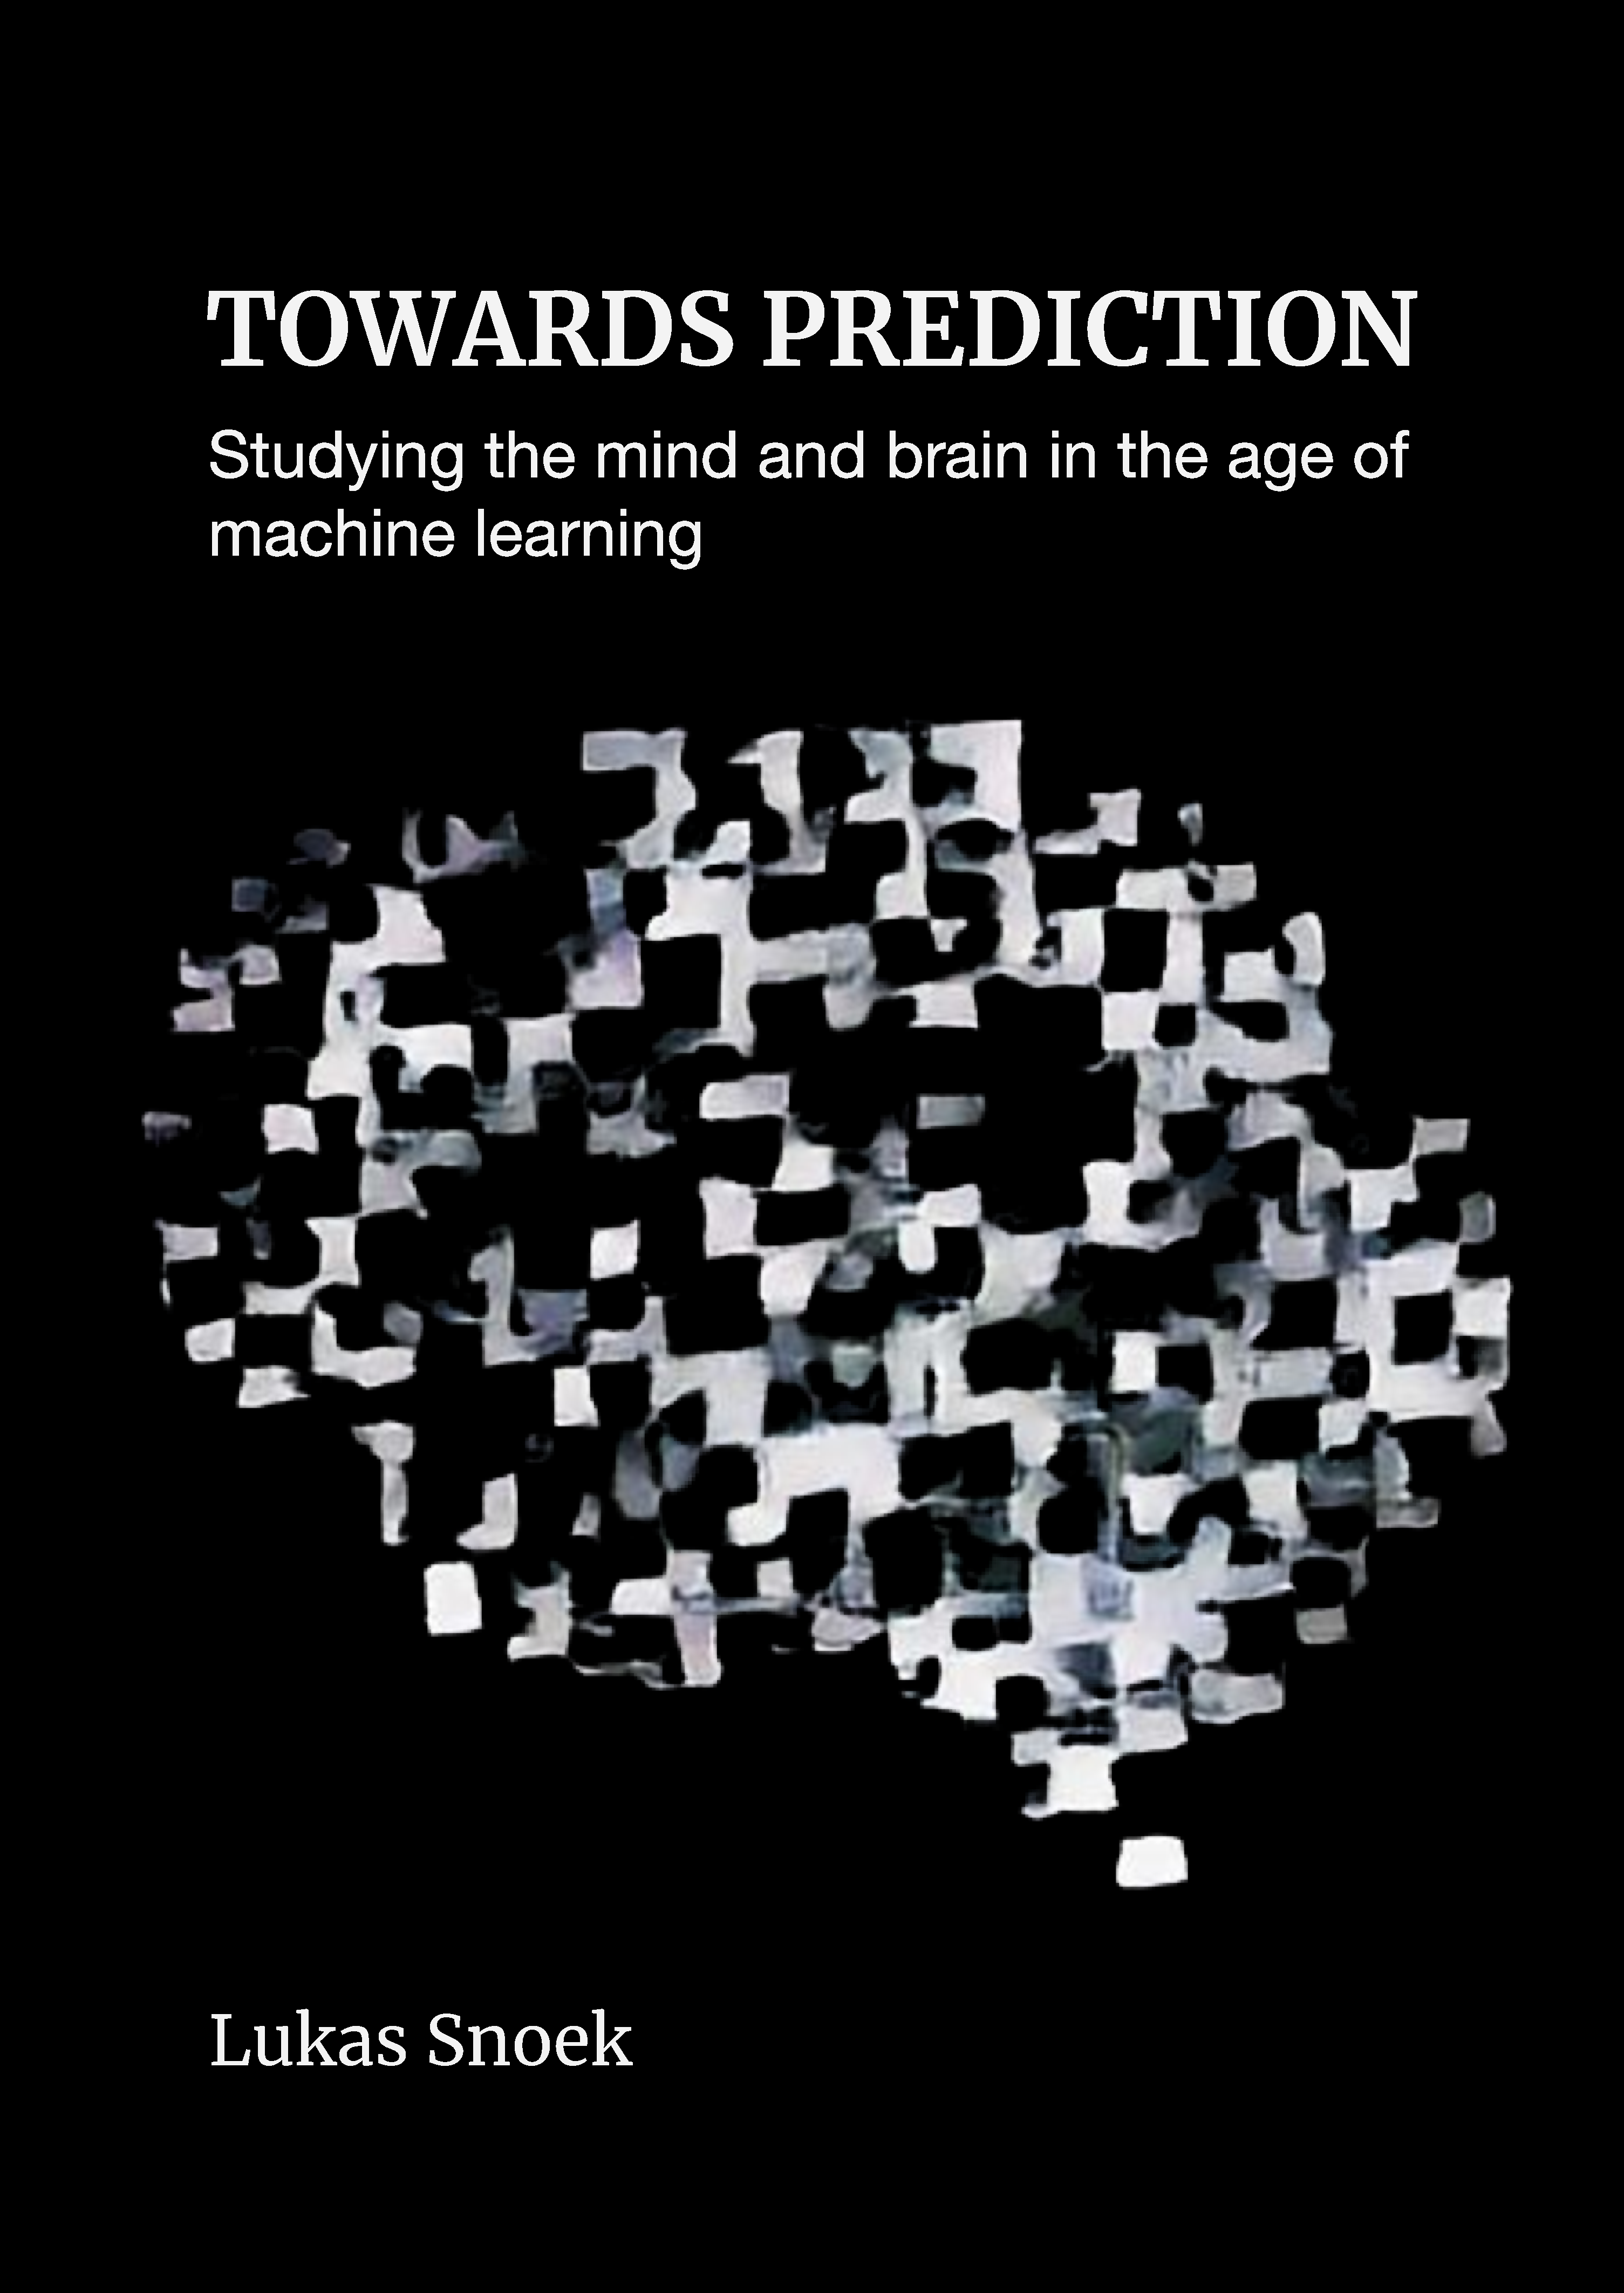
\includepdf{./cover/thesis_cover.pdf}

% \newlength{\mylen}                % a length
% \newcommand{\alphabet}{abcdefghijklmnopqrstuvwxyz} % the lowercase alphabet
% \begingroup                       % keep font change local% font specification e.g., \Large\sffamily
% \settowidth{\mylen}{\alphabet}
% The length of this alphabet is \the\mylen. % print in document\typeout{The length of the Large sans alphabetis \the\mylen}                    % put in log file
% \endgroup                         % end the grouping

{
\setcounter{tocdepth}{1}
\tableofcontents
}
\mainmatter
\hypertarget{introduction}{%
\chapter{Introduction}\label{introduction}}

\emph{The first chapter of the thesis, which introduces your PhD project. The filler-text below was created with the \href{http://www.elsewhere.org/journal/pomo}{postmodernism generator}.}

\begin{center}\rule{0.5\linewidth}{0.5pt}\end{center}

Something about the coming about of this thesis. More of a ``lessons learned'' rather than a coherent research topic.

\hypertarget{the-brain-is-not-a-dictionary}{%
\section{The brain is not a dictionary}\label{the-brain-is-not-a-dictionary}}

Something about looking at populations of neurons/voxels/areas rather than simple one-to-one relationships. Shared states.

\hypertarget{the-brain-probably-does-not-care-about-your-hypothesis}{%
\section{The brain (probably) does not care about your hypothesis}\label{the-brain-probably-does-not-care-about-your-hypothesis}}

Facial expression models.

\hypertarget{interpretability-and-prediction-are-a-trade-off-for-now}{%
\section{Interpretability and prediction are a trade-off (for now)}\label{interpretability-and-prediction-are-a-trade-off-for-now}}

A plea for prediction but a cautionary tale for interpreting predictive models (confounds)

\hypertarget{exploration-should-be-embraced-more}{%
\section{Exploration should be embraced more}\label{exploration-should-be-embraced-more}}

Something about the ``context of discovery'' (cf.~TCM), preregistration, and confirmation vs.~exploration (Morbid curiosity.)

\hypertarget{proper-generalization-is-hard}{%
\section{Proper generalization is hard}\label{proper-generalization-is-hard}}

Within and between subject variance is not noise, but unexplained variance (AU limitations).

\hypertarget{psychology-is-complex-so-it-needs-complex-models}{%
\section{Psychology is complex, so it needs complex models}\label{psychology-is-complex-so-it-needs-complex-models}}

Which need to be fit on complex, large datasets. (AOMIC)

\hypertarget{shared-states}{%
\chapter{Shared states: using MVPA to test neural overlap between self-focused emotion imagery and other-focused emotion understanding}\label{shared-states}}

\chaptermark{Shared states}

\vspace*{\fill}

\begin{center}\rule{0.5\linewidth}{0.5pt}\end{center}

\small

\noindent
\emph{This chapter has been published as}: Oosterwijk, S.*, Snoek, L.*, Rotteveel, M., Barrett, L. F., \& Scholte, H. S. (2017). Shared states: using MVPA to test neural overlap between self-focused emotion imagery and other-focused emotion understanding. \emph{Social cognitive and affective neuroscience, 12}(7), 1025-1035.

* Shared first authorship
\newpage
\normalsize

\textbf{Abstract}

The present study tested whether the neural patterns that support imagining ``performing an action'', ``feeling a bodily sensation'' or ``being in a situation'' are directly involved in understanding \emph{other people's} actions, bodily sensations and situations. Subjects imagined the content of short sentences describing emotional actions, interoceptive sensations and situations (self-focused task), and processed scenes and focused on \emph{how} the target person was expressing an emotion, \emph{what} this person was feeling, and \emph{why} this person was feeling an emotion (other-focused task). Using a linear support vector machine classifier on brain-wide multi-voxel patterns, we accurately decoded each individual class in the self-focused task. When generalizing the classifier from the self-focused task to the other-focused task, we also accurately decoded whether subjects focused on the emotional actions, interoceptive sensations and situations of \emph{others}. These results show that the neural patterns that underlie self-imagined experience are involved in understanding the experience of other people. This supports the theoretical assumption that the basic components of emotion experience and understanding share resources in the brain.

\hypertarget{Sharedstates-introduction}{%
\section{Introduction}\label{Sharedstates-introduction}}

To navigate the social world successfully it is crucial to understand other people. But how do people generate meaningful representations of other people's actions, sensations, thoughts and emotions? The dominant view assumes that representations of other people's experiences are supported by the same neural systems as those that are involved in generating experience in the self \autocites[e.g.,][]{gallese2004unifying}[see for an overview][]{singer2012past}. We tested this principle of self-other neural overlap directly, using multi-voxel pattern analysis (MVPA), across three different aspects of experience that are central to emotions: actions, sensations from the body and situational knowledge.

In recent years, evidence has accumulated that suggests a similarity between the neural patterns representing the self and others. For example, a great variety of studies have shown that observing actions and sensations in other people engages similar neural circuits as acting and feeling in the self \autocite[see for an overview][]{bastiaansen2009evidence}. Moreover, an extensive research program on pain has demonstrated an overlap between the experience of physical pain and the observation of pain in other people, utilizing both neuroimaging techniques \autocite[e.g.,][]{lamm2011meta} and analgesic interventions \autocites[e.g.,][]{rutgen2015placebo}{mischkowski2016painkiller}. This process of ``vicarious experience'' or ``simulation'' is viewed as an important component of empathy \autocite{carr2003neural,decety2011dissecting,keysers2014dissociating}. In addition, it is argued that mentalizing (e.g.~understanding the mental states of other people) involves the same brain networks as those involved in self-generated thoughts \autocite{uddin2007self,waytz2011two}. Specifying this idea further, a constructionist view on emotion proposes that both emotion experience and interpersonal emotion understanding are produced by the same large-scale distributed brain networks that support the processing of sensorimotor, interoceptive and situationally relevant information \autocite{barrett2013large,oosterwijk2014embodiment}. An implication of these views is that the representation of self- and other-focused emotional actions, interoceptive sensations and situations overlap in the brain.

Although there is experimental and theoretical support for the idea of self-other neural overlap, the present study is the first to directly test this process using MVPA across three different aspects of experience (i.e.~actions, interoceptive sensations and situational knowledge). Our experimental design consisted of two different tasks aimed at generating self- and other-focused representations with a relatively large weight given to either action information, interoceptive information or situational information.

In the \emph{self-focused} emotion imagery task (SF-task) subjects imagined performing or experiencing actions (e.g., \emph{pushing someone away}), interoceptive sensations (e.g., \emph{increased heart rate}) and situations (e.g., \emph{alone in a park at night}) associated with emotion. Previous research has demonstrated that processing linguistic descriptions of (emotional) actions and feeling states can result in neural patterns of activation associated with, respectively, the representation and generation of actions and internal states \autocite{pulvermuller2010active,oosterwijk2015concepts}. Furthermore, imagery-based inductions of emotion have been successfully used in the MRI scanner before \autocite{wilson2011grounding,oosterwijk2012states}, and are seen as robust inducers of emotional experience \autocite{lench2011discrete}. In the \emph{other-focused} emotion understanding task (OF-task), subjects viewed images of people in emotional situations and focused on actions (i.e., \emph{How} does this person express his/her emotions?), interoceptive sensations (i.e., \emph{What} does this person feel in his/her body) or the situation (i.e., \emph{Why} does this person feel an emotion?). This task is based on previous research studying the neural basis of emotion oriented mentalizing \autocite{spunt2012integrative}.

With MVPA, we examined to what extent the SF- and OF-task evoked similar neural patterns. MVPA allows researchers to assess whether the neural pattern associated with one set of experimental conditions can be used to distinguish between another set of experimental conditions. This relatively novel technique has been successfully applied to the field of social neuroscience in general \autocites[e.g.,][]{gilbert2012evaluative}{brosch2013implicit}{parkinson2014common}, and the field of self-other neural overlap in particular. For example, several MVPA studies recently assessed whether experiencing pain and observing pain in others involved similar neural patterns \autocite{corradi2016cross,krishnan2016somatic}. Although there is an ongoing discussion about the specifics of shared representation in pain based on these MVPA results \autocite[see for an overview][]{zaki2016anatomy}, many authors emphasize the importance of this technique in the scientific study of self-other neural overlap \autocites[e.g.,][]{corradi2016cross}{krishnan2016somatic}.

MVPA is an analysis technique that decodes latent categories from fMRI data in terms of multi-voxel patterns of activity \autocite{norman2006beyond}. This technique is particularly suited for our research question for several reasons. First of all, although univariate techniques can demonstrate that tasks activate the same brain regions, only MVPA can statistically test for shared representation \autocite{lamm2015role}. We will evaluate whether multivariate brain patterns that distinguish between mental events in the SF-task can be used to distinguish, above chance level, between mental events in the OF-task. Second, MVPA analyses are particularly useful in research that is aimed at examining distributed representations \autocite{singer2012past}. Based on our constructionist framework, we indeed hypothesize that the neural patterns that will represent self- and other focused mental events are distributed across large-scale brain networks. To capture these distributed patterns, we used MVPA in combination with data-driven univariate feature selection on whole-brain voxel patterns, instead of limiting our analysis to specific regions-of-interest \autocite{haynes2015primer}. And third, in contrast to univariate analyses that aggregate data across subjects, MVPA can be performed within-subjects and is thus able to incorporate individual variation in the representational content of multivariate brain patterns. In that aspect within-subject MVPA is sensitive to individual differences in how people imagine actions, sensations and situations, and how they understand others. In short, for our purpose to explicitly test the assumption that self and other focused processes share neural resources, MVPA is the designated method.

We tested the following two hypotheses. First, we tested whether we could classify \emph{self-imagined} actions, interoceptive sensations and situations above chance level. Second, we tested whether the multivariate pattern underlying this classification could also be used to classify the how, what and why condition in the \emph{other-focused} task.

\hypertarget{Sharedstates-methods}{%
\section{Methods}\label{Sharedstates-methods}}

\hypertarget{subjects}{%
\subsection{Subjects}\label{subjects}}

In total, we tested 22 Dutch undergraduate students from the University of Amsterdam (14 females; M\textsubscript{age} = 21.48, s.d.\textsubscript{age} = 1.75). Of those 22 subjects, 13 subjects were tested twice in 2 sessions about 1 week apart. Half of those sessions were used for the model optimization procedure. The other half of the sessions, combined with an additional nine subjects (who were tested only once), constituted the model validation set (see Model optimization procedure section). In total, two subjects were excluded from the model validation dataset: one subject was excluded because there was not enough time to complete the experimental protocol and another subject was excluded due to excessive movement (\textgreater3 mm within data acquisition runs).

All subjects signed informed consent prior to the experiment. The experiment was approved by the University of Amsterdam's ethical review board. Subjects received 22.50 euro per session. Standard exclusion criteria regarding MRI safety were applied and people who were on psychopharmacological medication were excluded a priori.

\hypertarget{experimental-design}{%
\subsection{Experimental design}\label{experimental-design}}

\hypertarget{self-focused-emotion-imagery-task}{%
\subsubsection{Self-focused emotion imagery task}\label{self-focused-emotion-imagery-task}}

The self-focused emotion imagery task (SF-task) was created to preferentially elicit \emph{self-focused} processing of action, interoceptive or situational information associated with emotion. Subjects processed short linguistic cues that described actions (e.g., \emph{pushing someone away}; \emph{making a fist}), interoceptive sensations (e.g., \emph{being out of breath}; \emph{an increased heart rate}), or situations (e.g., \emph{alone in a park at night}; \emph{being falsely accused}) and were instructed to imagine performing or experiencing the content. The complete instruction is presented in the Supplementary Materials; all stimuli used in the SF-task are presented in Supplementary Table S1. Linguistic cues were selected from a pilot study performed on an independent sample of subjects (\emph{n} = 24). Details about this pilot study are available on request. The descriptions generated in this pilot study were used as qualitative input to create short sentences that described actions, sensations or situations that were associated with negative emotions, without including discrete emotion terms. The cues did not differ in number of words, nor in number of characters (\emph{F} \textless{} 1).

\hypertarget{confounds-decoding}{%
\chapter{How to control for confounds in decoding analyses of neuroimaging data}\label{confounds-decoding}}

\hypertarget{AOMIC}{%
\chapter{The Amsterdam Open MRI Collection, a set of multimodal MRI datasets for individual difference analyses}\label{AOMIC}}

\hypertarget{morbid-curiosity}{%
\chapter{Choosing to view morbid information involves reward circuitry}\label{morbid-curiosity}}

\hypertarget{au-limitations}{%
\chapter{Using predictive modeling to quantify the importance and limitations of action units in emotion perception}\label{au-limitations}}

\hypertarget{facial-expression-models}{%
\chapter{Comparing models of dynamic facial expression perception}\label{facial-expression-models}}

\hypertarget{summary-and-general-discussion}{%
\chapter{Summary and general discussion}\label{summary-and-general-discussion}}

My view on going forward.

\hypertarget{explore}{%
\section{Explore!}\label{explore}}

Theories are like toothbrushes, no one likes to use someone else's.

\hypertarget{think-big}{%
\section{\texorpdfstring{Think \emph{big}}{Think big}}\label{think-big}}

Big, complex datasets to train big, complex models.

\hypertarget{rethink-psychology-education}{%
\section{Rethink psychology education}\label{rethink-psychology-education}}

Embrace and teach interdisciplinary.

\hypertarget{appendix-appendix}{%
\appendix}


\cleardoublepage
\phantomsection
\addcontentsline{toc}{part}{Appendices}
\appendixpage*
\setlength\beforechapskip{-\baselineskip}

\hypertarget{shared-states-supplement}{%
\chapter{Supplement to Chapter \ref{shared-states}}\label{shared-states-supplement}}

\hypertarget{stimuli-used-for-sf-task}{%
\section{Stimuli used for SF-task}\label{stimuli-used-for-sf-task}}

\begin{table}

\caption{\label{tab:tab-shared-states-S1}Stimuli used for SF-task}
\centering
\resizebox{\linewidth}{!}{
\begin{tabular}[t]{lll}
\toprule
Class & Dutch & English translation\\
\midrule
Action & Hard wegrennen & Running away fast\\
 & Iemand wegduwen & Pushing someone away\\
 & Iemand stevig vastpakken & Holding someone tightly\\
 & Je hoofd schudden & Shaking your head\\
 & Heftige armgebaren maken & Making big arm gestures\\
\addlinespace
 & Ergens voor terugdeinzen & Recoiling from something\\
 & Je ogen dichtknijpen & Closing your eyes tightly\\
 & Je ogen wijd open sperren & Opening your eyes widely\\
 & Je wenkbrauwen fronsen & Frowning with your eyebrows\\
 & Je schouders ophalen & Raising your shoulders\\
\addlinespace
 & Op de vloer stampen & Stamping on the floor\\
 & In elkaar duiken & Cowering\\
 & Je schouders laten hangen & Slumping your shoulders\\
 & Je vuisten ballen & Tighten your fists\\
 & Je borst vooruit duwen & Push your chest forward\\
\addlinespace
 & Je tanden op elkaar zetten & Clench your teeth\\
 & Je hand voor je mond slaan & Put your hand in front of your mouth\\
 & Onrustig bewegen & Moving restlessly\\
 & Heen en weer lopen & Walking back and forth\\
 & Je hoofd afkeren & Turning your head away\\
\addlinespace
Interoception & Een brok in je keel & A lump in your throat\\
 & Buiten adem zijn & Being out of breath\\
 & Een versnelde hartslag & A fast beating heart\\
 & Je hart klopt in de keel & You heart is beating in your throat\\
 & Een benauwd gevoel & An oppressed feeling\\
\addlinespace
 & Een misselijk gevoel & Being nauseous\\
 & Druk op je borst & A pressure on your chest\\
 & Strak aangespannen spieren & Tense muscles\\
 & Een droge keel & A dry throat\\
 & Koude rillingen hebben & Cold shivers\\
\addlinespace
 & Bloed stroomt naar je hoofd & Blood is going to your head\\
 & Een verdoofd gevoel & A numb feeling\\
 & Je hebt tintelende ledenmaten & Tingling limbs\\
 & Een verlaagde hartslag & A slow heartbeat\\
 & Je hebt zware ledematen & Heavy limbs\\
\addlinespace
 & Een versnelde ademhaling & Fast breathing\\
 & Je hebt hoofdpijn & Headache\\
 & Je hebt buikpijn & Stomachache\\
 & Zweet staat in je handen & Sweaty palms\\
 & Je maag keert zich om & Your stomach churns\\
\addlinespace
Situation & Vals beschuldigd worden & Being falsely accused\\
 & Dierbare overlijdt & A loved one dies\\
 & Vlees is bedorven & Meat that has gone off\\
 & Je wordt bijna aangereden & You are almost hit by a car\\
 & Iemand naast je braakt & Someone next to you vomits\\
\addlinespace
 & Huis staat in brand & House is on fire\\
 & Zonder reden ontslagen worden & Being fired for no reason\\
 & Een ongemakkelijke stilte & An uncomfortable silence\\
 & Alleen in donker park & Alone in a dark park\\
 & Inbraak in je huis & A house burglary\\
\addlinespace
 & Een gewond dier zien & Seeing a wounded animal\\
 & Tentamen verknallen & Messing up your exam\\
 & Je partner bedriegt je & You partner cheats on you\\
 & Dierbare is vermist & A loved one is missing\\
 & Belangrijke sollicitatie vergeten & Forgot a job interview\\
\addlinespace
 & Onvoorbereid presentatie geven & Giving a presentation unprepared\\
 & Je baas beledigt je & Your boss offends you\\
 & Goede vriend negeert je & A good friend neglects you\\
 & Slecht nieuws bij arts & Bad news at the doctor\\
 & Bommelding in metro & A bomb alarm in the metro\\
\bottomrule
\multicolumn{3}{l}{\rule{0pt}{1em}\textit{Note: } The stimulus materials presented in Table S1 were selected from a pilot study. In this pilot study we asked an independent sample of twenty-four subjects to describe how they would express an emotion in their behavior, body posture or facial expression (action information), what specific sensations they would feel inside their body when they would experience an emotion (interoceptive information), and for what reason or in what situation they would experience an emotion (situational information). These three questions were asked in random order for twenty-eight different negative emotional states, including anger, fear, disgust, sadness, contempt, worry, disappointment, regret and shame. The descriptions generated by these subjects were used as qualitative input in order to create our stimulus set of twenty short sentences that described emotional actions, sensations or situations. With this procedure, we ensured that our stimulus set held sentences that were validated and ecologically appropriate for our sample.}\\
\end{tabular}}
\end{table}

\hypertarget{full-instruction-for-the-other-focused-emotion-understanding-task}{%
\section{Full instruction for the other-focused emotion understanding task}\label{full-instruction-for-the-other-focused-emotion-understanding-task}}

\emph{Translated from Dutch; task presented first.}

In this study we are interested in how the brain responds when people understand the emotions of others in different ways. In the scanner you will see images that display emotional situations, sometimes with multiple people. In every image one person will be marked with a red square. While viewing the image we ask you to focus on the emotion of that person in three different ways.

With some images we ask you to focus on HOW this person expresses his or her emotion. Here we ask you to identify expressions in the face or body that are informative about the emotional state that the person is experiencing.

With other images we ask you to focus on WHAT this person may feel in his or her body. Here we ask you to identify sensations, such as a change in heart rate, breathing or other internal feeling, that the person might feel in this situation.

With other images we ask you to focus on WHY this person experiences an emotion. Here we ask you to identify a specific reason or cause that explains why the person feels what he or she feels.

Every image will be presented for six seconds. During this period we ask you to silently focus on HOW this person expresses emotion, WHAT this person feels in his/her body, and WHY this person feels an emotion.

Before you will enter the scanner we will practice. I will show you three images and will ask you to perform each of the three instructions out loud.

It is important to note that there are no correct or incorrect answers, it is about how you interpret the image. For the success of the study it is very important that you apply the HOW, WHAT or WHY instruction for each image. Please do not skip any images and try to apply each instruction with the same motivation. It is also important to treat every image separately, although it is possible that you have similar interpretations for different images.

The three instructions are combined with the images in blocks. In every block you will see five images with the same instruction. Each block will start with a cue that tells you what to focus on in that block.

Each image is combined with all three instructions, so you will see the same image multiple times. In between images you will sometimes see a black screen for a longer period of time.

Do you have any questions?

\newpage
\pagestyle{empty}

\hypertarget{full-instruction-for-the-self-focused-emotion-imagery-task}{%
\section{Full instruction for the self-focused emotion imagery task}\label{full-instruction-for-the-self-focused-emotion-imagery-task}}

\emph{Translated from Dutch; task presented second.}

In this study we are interested in how the brain responds when people imagine different aspects of emotion. In the scanner you will see sentences that describe aspects of emotional experience. We ask you to try to imagine the content of each sentence as rich and detailed as possible.

Some sentences describe actions and expressions. We ask you to imagine that you are performing this action or expression. Other sentences describe sensations or feelings that you can have \emph{inside} your body. We ask you to imagine that you are experiencing this sensation or feeling. Other sentences describe emotional situations. We ask you to imagine that you are experiencing this specific situation.

We ask you to always imagine that YOU have the experience. Thus, it is about imagining an action or expression of your body, a sensation inside your body, or a situation that you are part of.

I will give some examples now.

For each sentence you have six seconds to imagine the content. All sentences will be presented twice. In between sentences you will sometimes see a black screen for a longer period of time. For this experiment to succeed it is important that you imagine each sentence with the same motivation, even if you have seen the sentence before. Please do not skip sentences.

Do you have any questions?

\newpage
\pagestyle{empty}

\begin{figure}
\centering
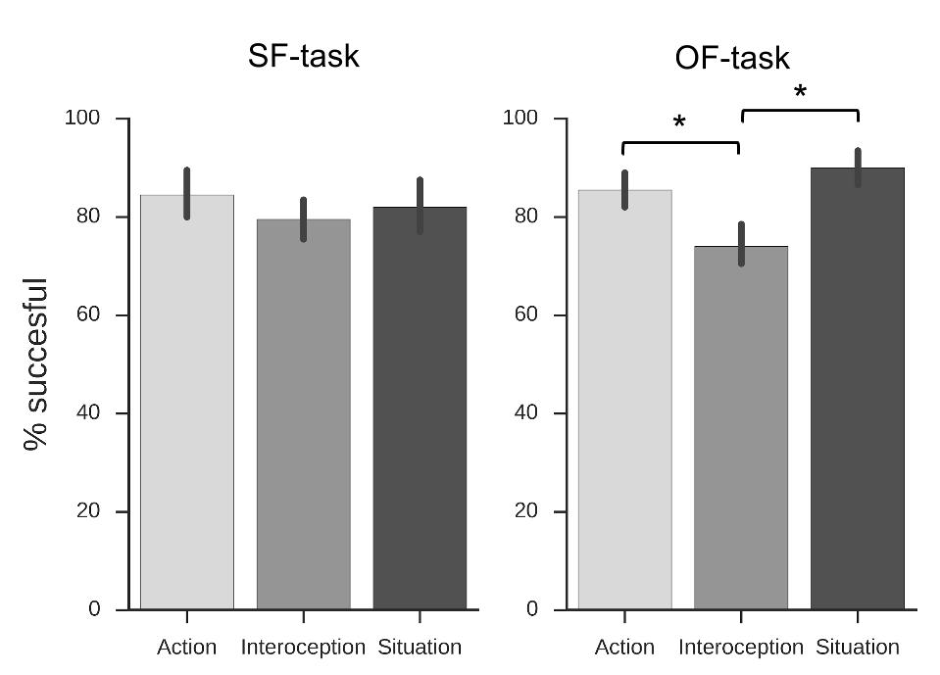
\includegraphics{_bookdown_files/shared-states-files/figures/figure_S1.pdf}
\caption{\label{fig:fig-shared-states-S1}Mean percentage of trials successfully executed for the SF-task (left panel) and OF-task (right panel). Error bars indicate 95\% confidence intervals. A one-way ANOVA of the success-rates of the SF-task (left-panel) indicated no significant overall differences, F(2, 17) = 1.03, p = 0.38. In the OF-task (right panel) however, a one-way ANOVA indicated that success-rates differed significantly between classes, F(2, 17) = 17.74, p \textless{} 0.001. Follow-up pairwise comparisons (Bonferroni corrected, two tailed) revealed that interoception-trials (M = 74.00, SE = 2.10) were significantly less successful (p \textless{} 0.001) than both action-trials (M = 85.50, SE = 1.85) and situation trials (M = 90.00, SE = 1.92).}
\end{figure}



\newpage
\pagestyle{empty}
\blandscape

\hypertarget{optimization-results}{%
\section{Optimization results}\label{optimization-results}}

\begin{figure}
\centering
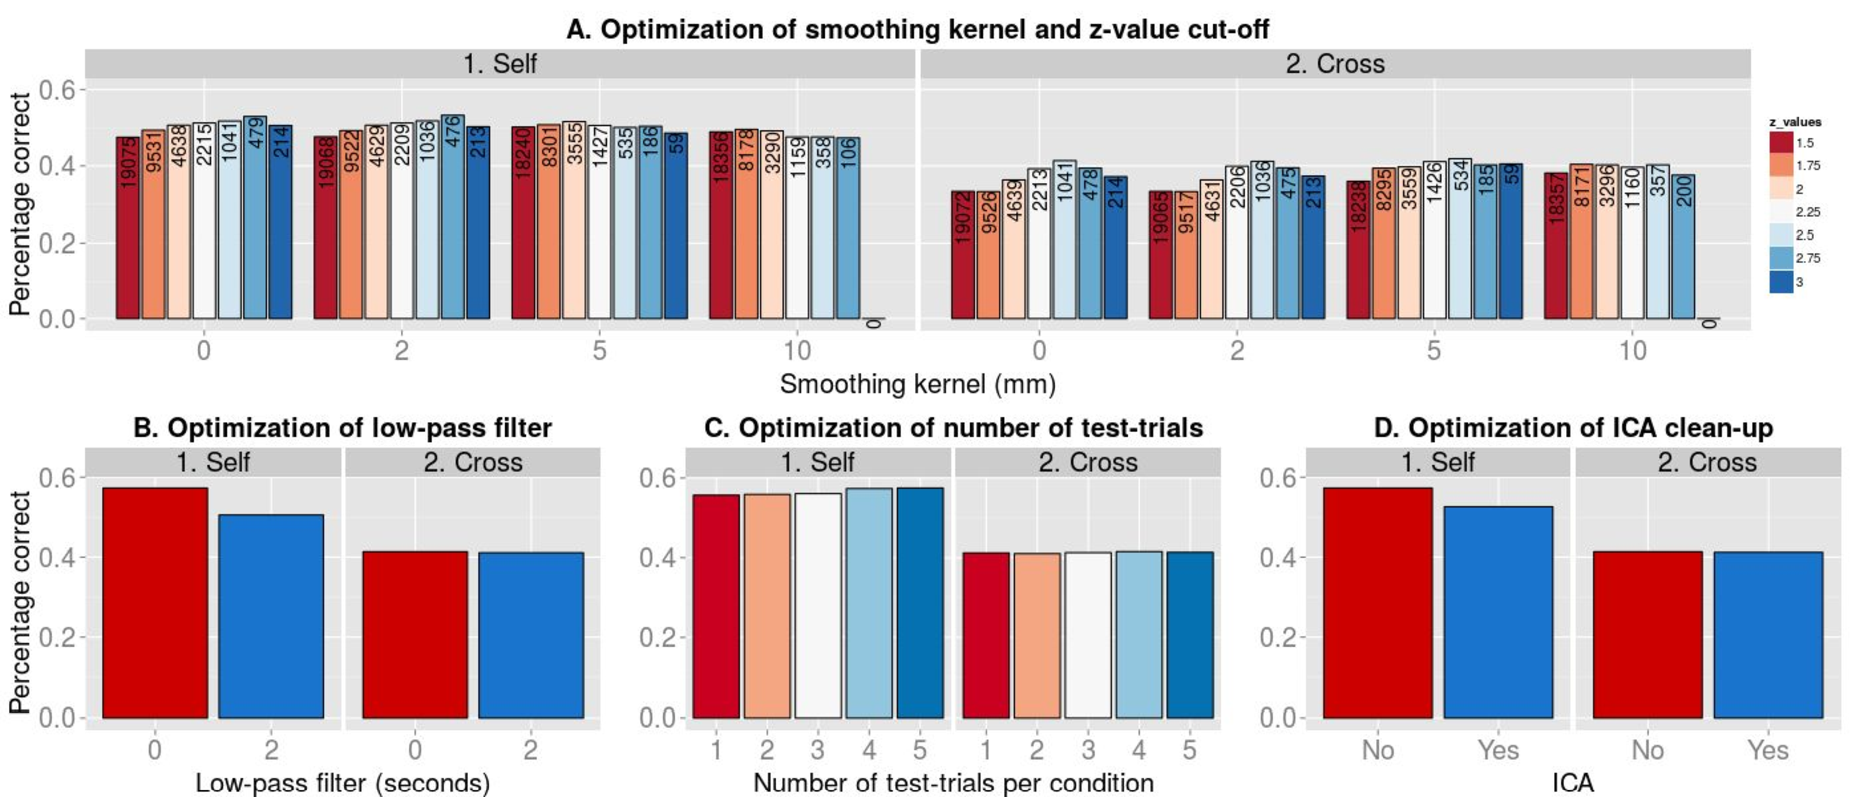
\includegraphics{_bookdown_files/shared-states-files/figures/figure_S2.pdf}
\caption{\label{fig:fig-shared-states-S2}Results of the parameter-optimization procedure. Reported scores reflect the classification scores averaged over subjects and classes (i.e.~the diagonal of the confusion matrix). All optimization analyses were iterated 5000 times. \textbf{A}) Classification results for different smoothing kernels (0, 2, 5, and 10 mm) and z-value threshold for differentiation scores during feature selection (see MVPA pipeline section in the main text for a description of the particular feature selection method we employed). Numbers reflect the average number of voxels selected across iterations. \textbf{B}) Classification results of using a low-pass filter (2 seconds) or not. \textbf{C}) Classification results for different numbers of test-trials per class (1 to 5). \textbf{D}) Classification results when preprocessing the data with Independent Component Analysis (ICA) or not.}
\end{figure}



\newpage
\elandscape

\begin{table}

\caption{\label{tab:tab-shared-states-S2}Parameters assessed in the optimization set.}
\centering
\resizebox{\linewidth}{!}{
\begin{tabular}[t]{lll}
\toprule
Parameter & Options & Final choice\\
\midrule
Smoothing kernel & 0 mm, 2 mm, 5 mm, 10 mm & 5 mm\\
Feature selection threshold & 1.5, 1.75, 2, 2.25, 2.5, 2.75, 3 & 2.2999999999999998\\
Number of test-trials & 1, 2, 3, 4, 5 & 4\\
Low-pass filter & 2 seconds vs. none & None\\
ICA denoising & ICA vs. no ICA & No ICA\\
\bottomrule
\multicolumn{3}{l}{\rule{0pt}{1em}\textit{Note: } The first set of parameters we evaluated in the optimization-set were different smoothing factors and feature selection thresholds (see MVPA pipeline section in the main text). On average, across the self- and cross-analysis, a 5 mm smoothing kernel yielded the best results in combination with a feature selection threshold of 2.25, which we rounded up to 2.3 as this number represents a normalized (z-transformed) score, which corresponds to the top 1\% scores within a normal distribution. Next, the difference between using a low-pass (of 2 seconds, i.e. 1 TR) versus none was assessed, establishing no low-pass filter as the optimal choice. Next, different numbers of test-trials (1 to 5) per class per iteration were assessed. Four trials yielded the best results. Lastly, the effect of “cleaning” the data with an independent component analysis was examined (FSL: MELODIC and FIX; Salimi-Khorshidi et al., 2014). Not performing ICA yielded the best results. These parameters – 5 mm smoothing kernel, 2.3 feature selection thresholded, no low-pass filter, and four test-trials per iteration – were subsequently used in the analysis of the validation set.}\\
\end{tabular}}
\end{table}

\newpage
\pagestyle{empty}

\begin{figure}
\centering
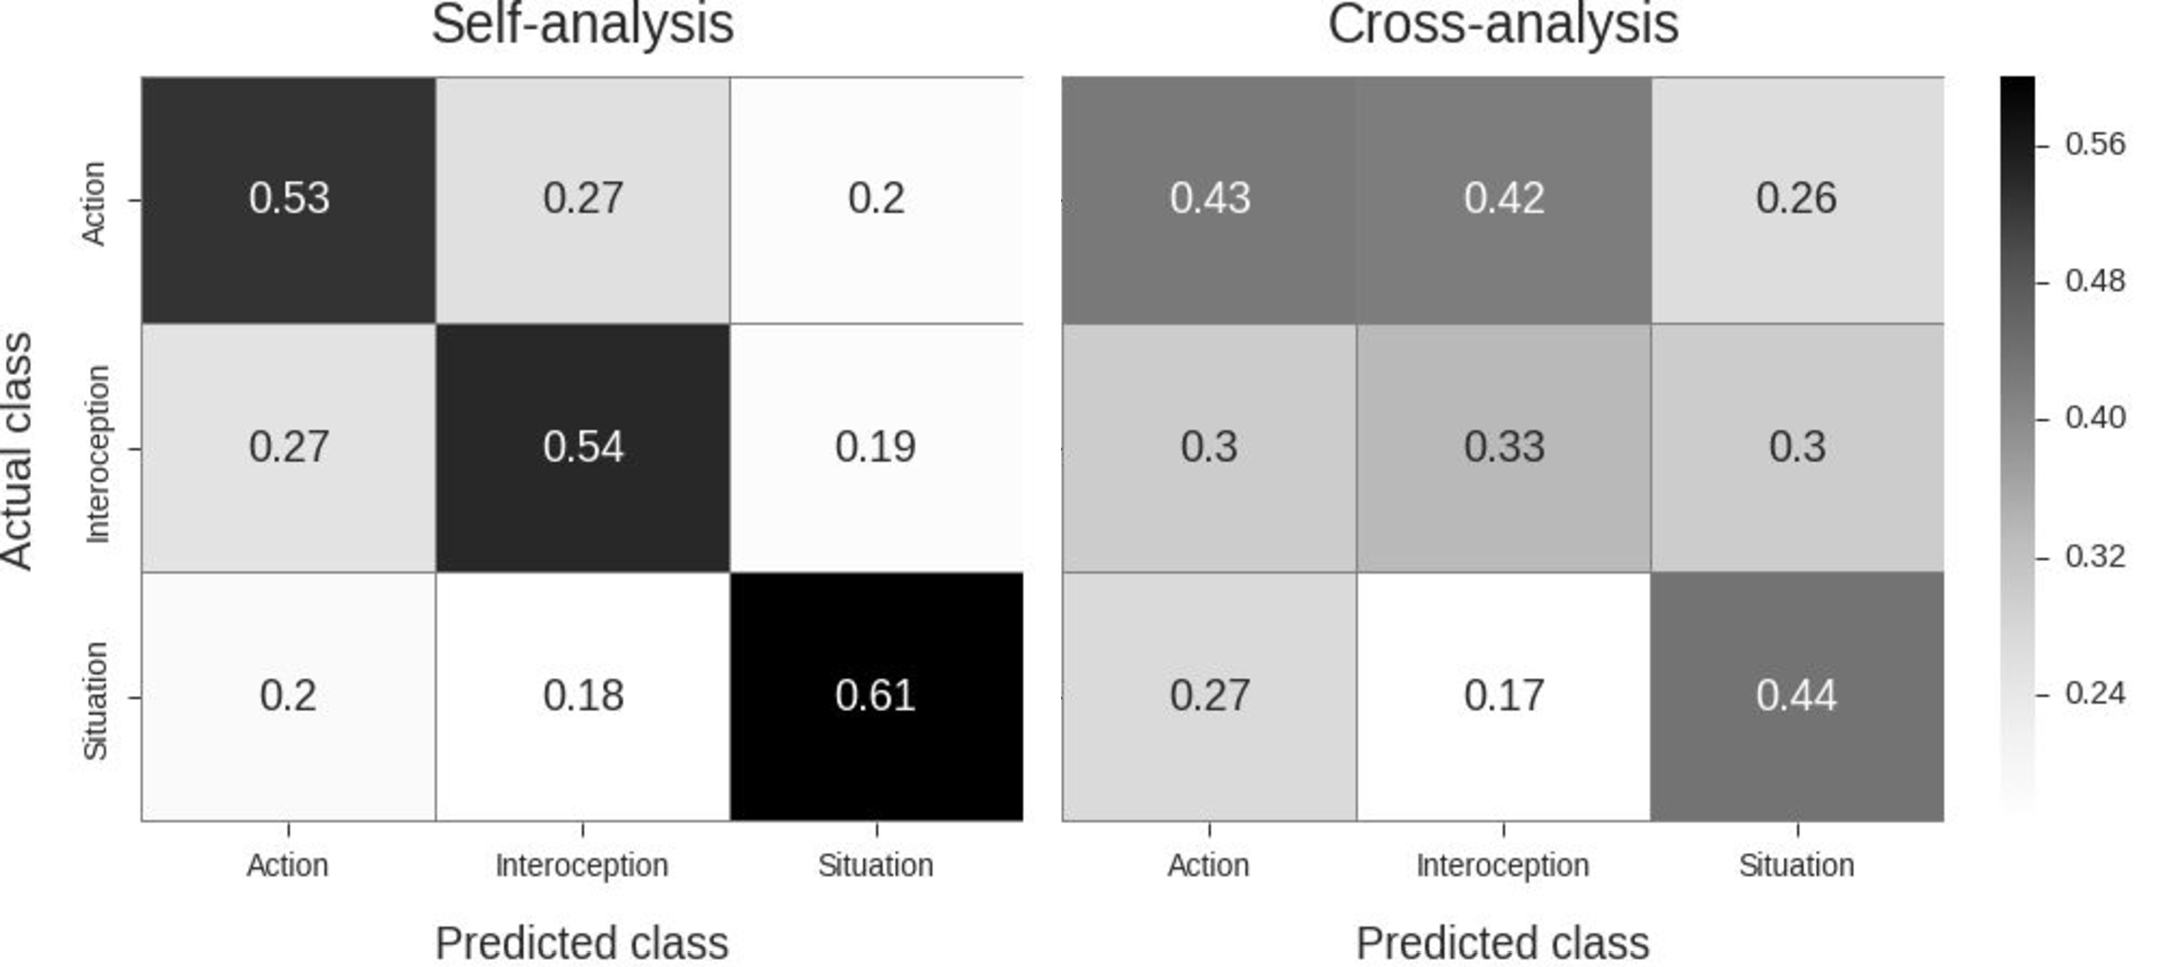
\includegraphics{_bookdown_files/shared-states-files/figures/figure_S3.pdf}
\caption{\label{fig:fig-shared-states-S3}Confusion matrices displaying precision-values yielded by the classification analysis of the optimization dataset with the final set of parameters. Because no permutation statistics were calculated for the optimization set, significance was calculated using a one-sample independent \emph{t}-test against chance-level classification (i.e.~0.333) for each cell in the diagonal of the confusion matrices. Here, all t-statistics use a degrees of freedom of 12 (i.e.~13 subjects - 1) and are evaluated against a significance level of 0.05, Bonferroni-corrected. For the diagonal of the self-analysis confusion matrix, all values were significantly above chance-level, all \emph{p} \textless{} 0.0001. For the diagonal of the cross-analysis confusion matrix, both the action (43\% correct) and situation (44\% correct) classes scored significantly above chance, \emph{p} = 0.014 and \emph{p} = 0.0007 respectively. Interoception was classified at chance level, \emph{p} = 0.99, which stands in contrast with the results in the validation-set.}
\end{figure}



\newpage
\pagestyle{empty}

\hypertarget{bagging-procedure}{%
\section{Bagging procedure}\label{bagging-procedure}}

\begin{figure}
\centering
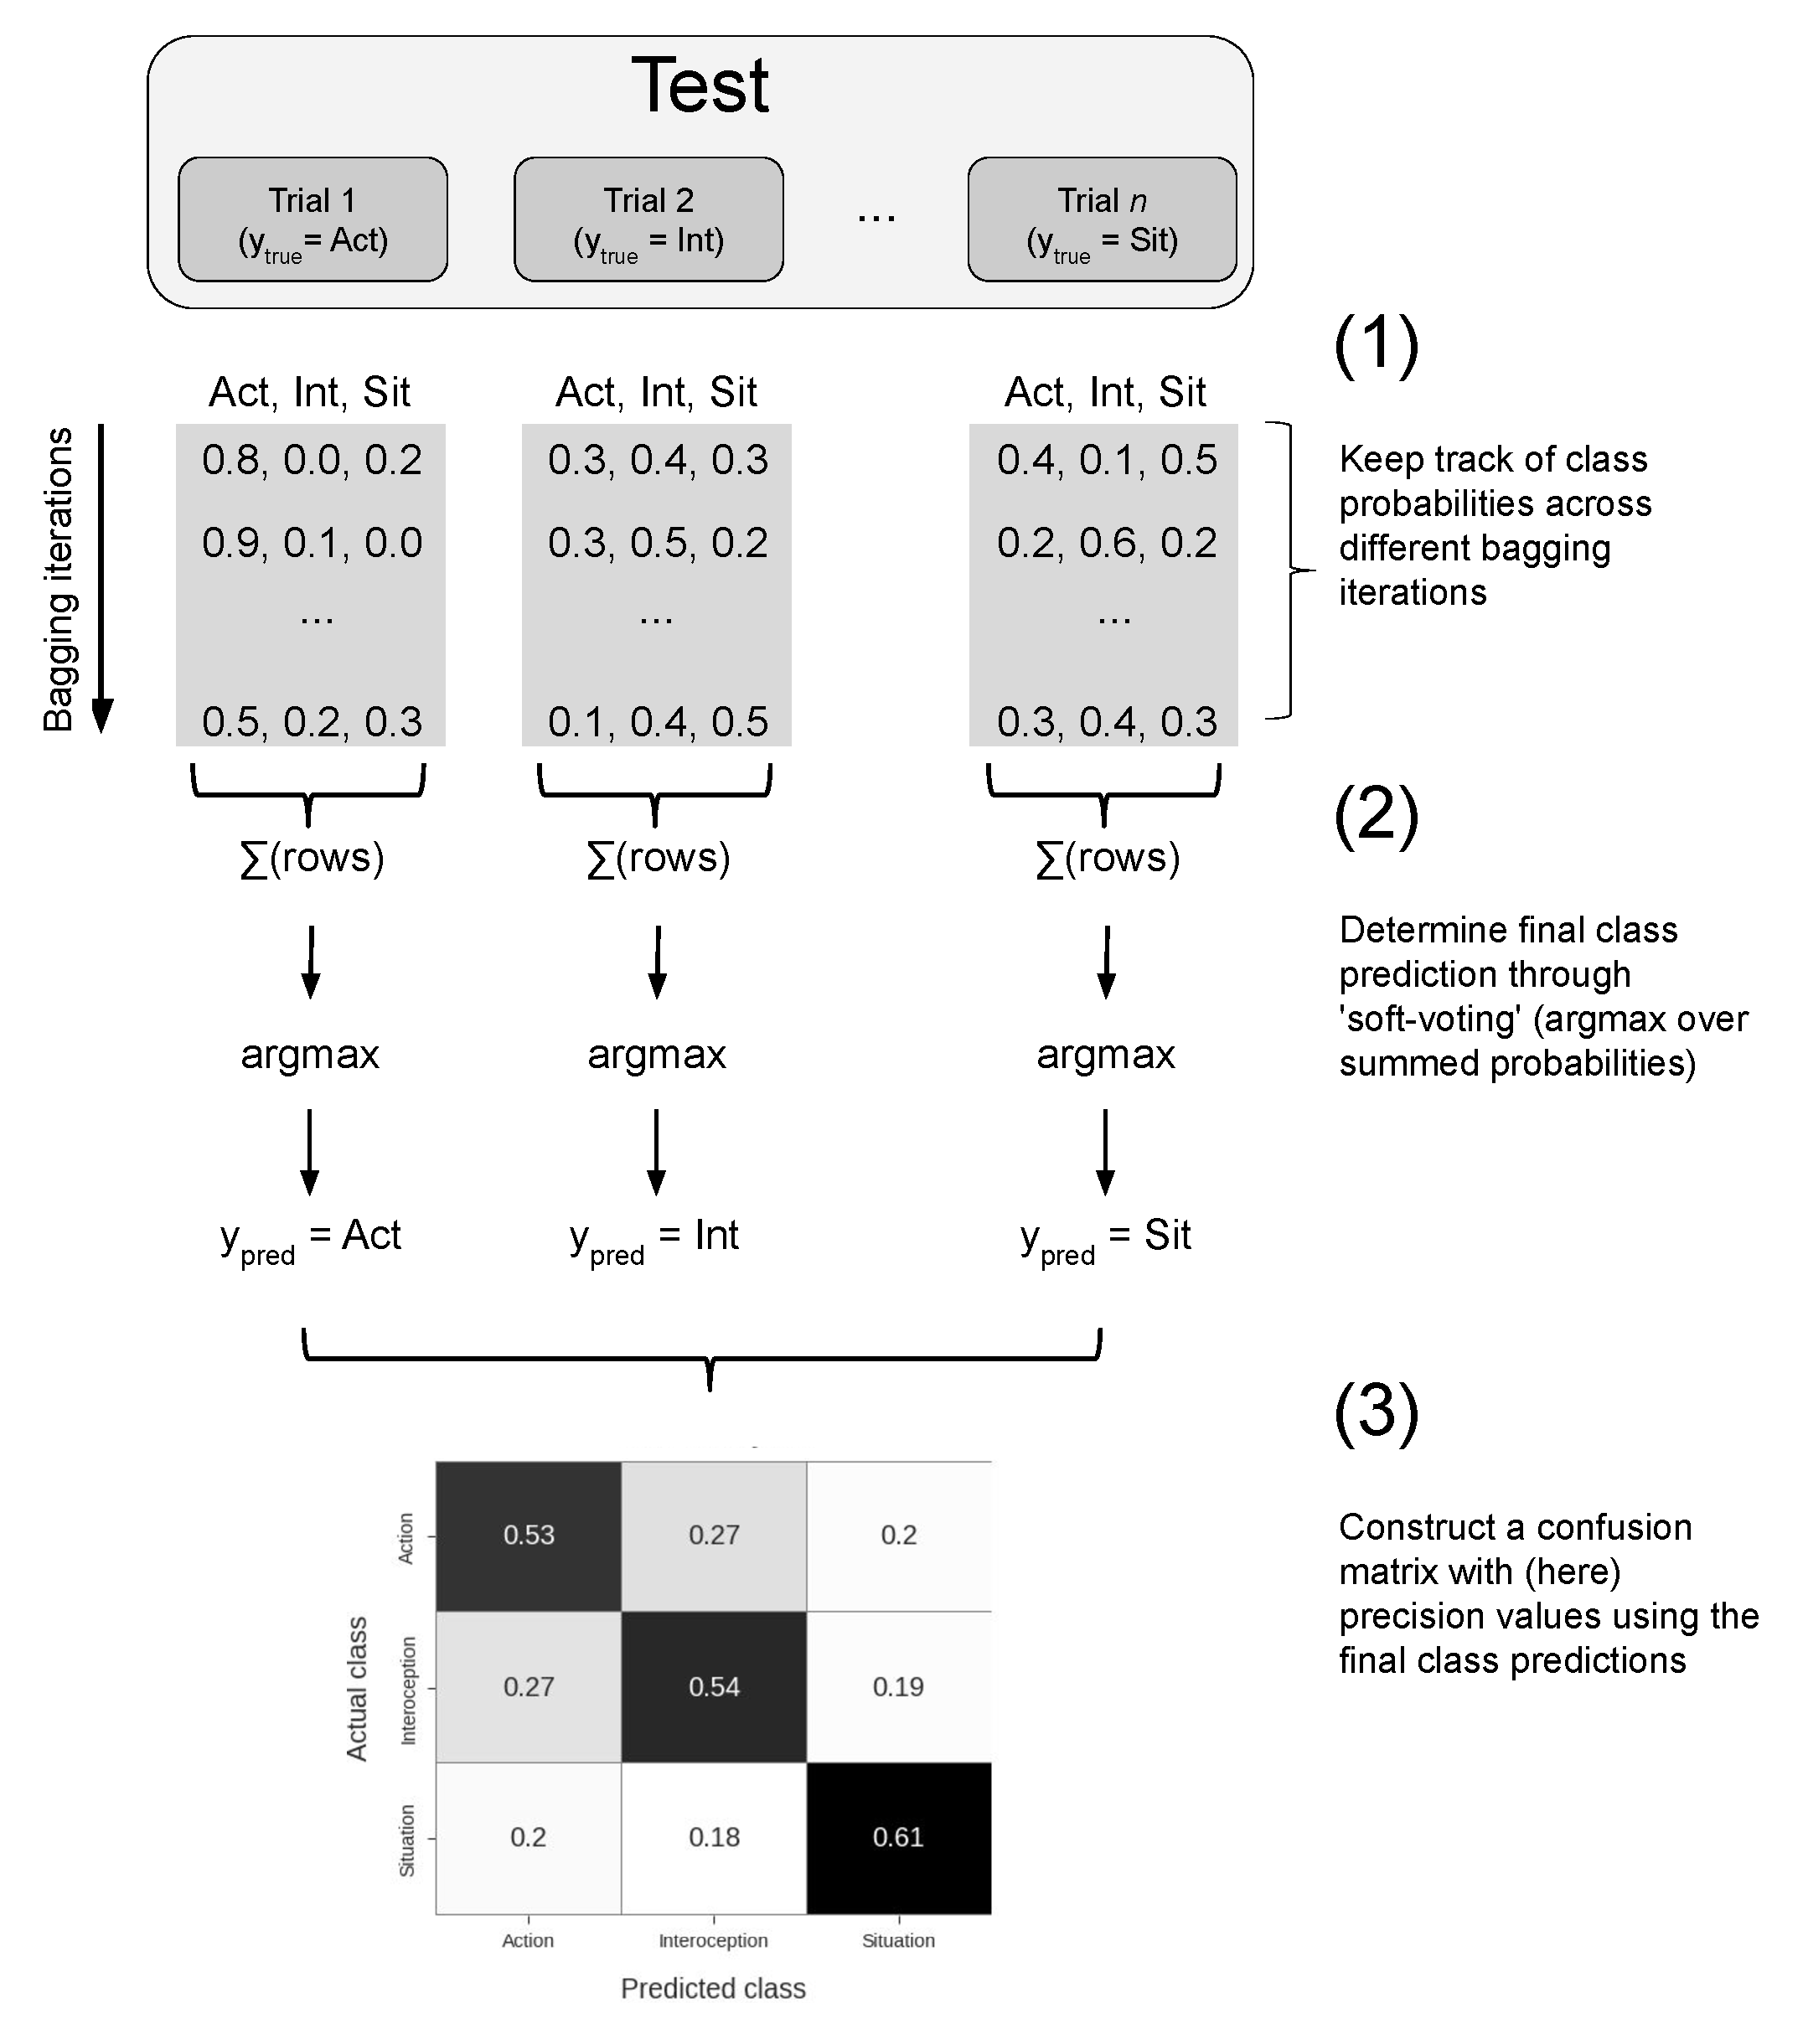
\includegraphics{_bookdown_files/shared-states-files/figures/figure_S4.pdf}
\caption{\label{fig:fig-shared-states-S4}Schematic overview of the bagging procedure. Class probabilities across different bagging iterations are summed and the class with the maximum probability determines each trial's final predicted class, which are subsequently summarized in a confusion matrix on which final recall/precision scores are calculated.}
\end{figure}



\newpage
\pagestyle{empty}

\hypertarget{precision-vs.-recall}{%
\section{Precision vs.~recall}\label{precision-vs.-recall}}

\begin{figure}
\centering
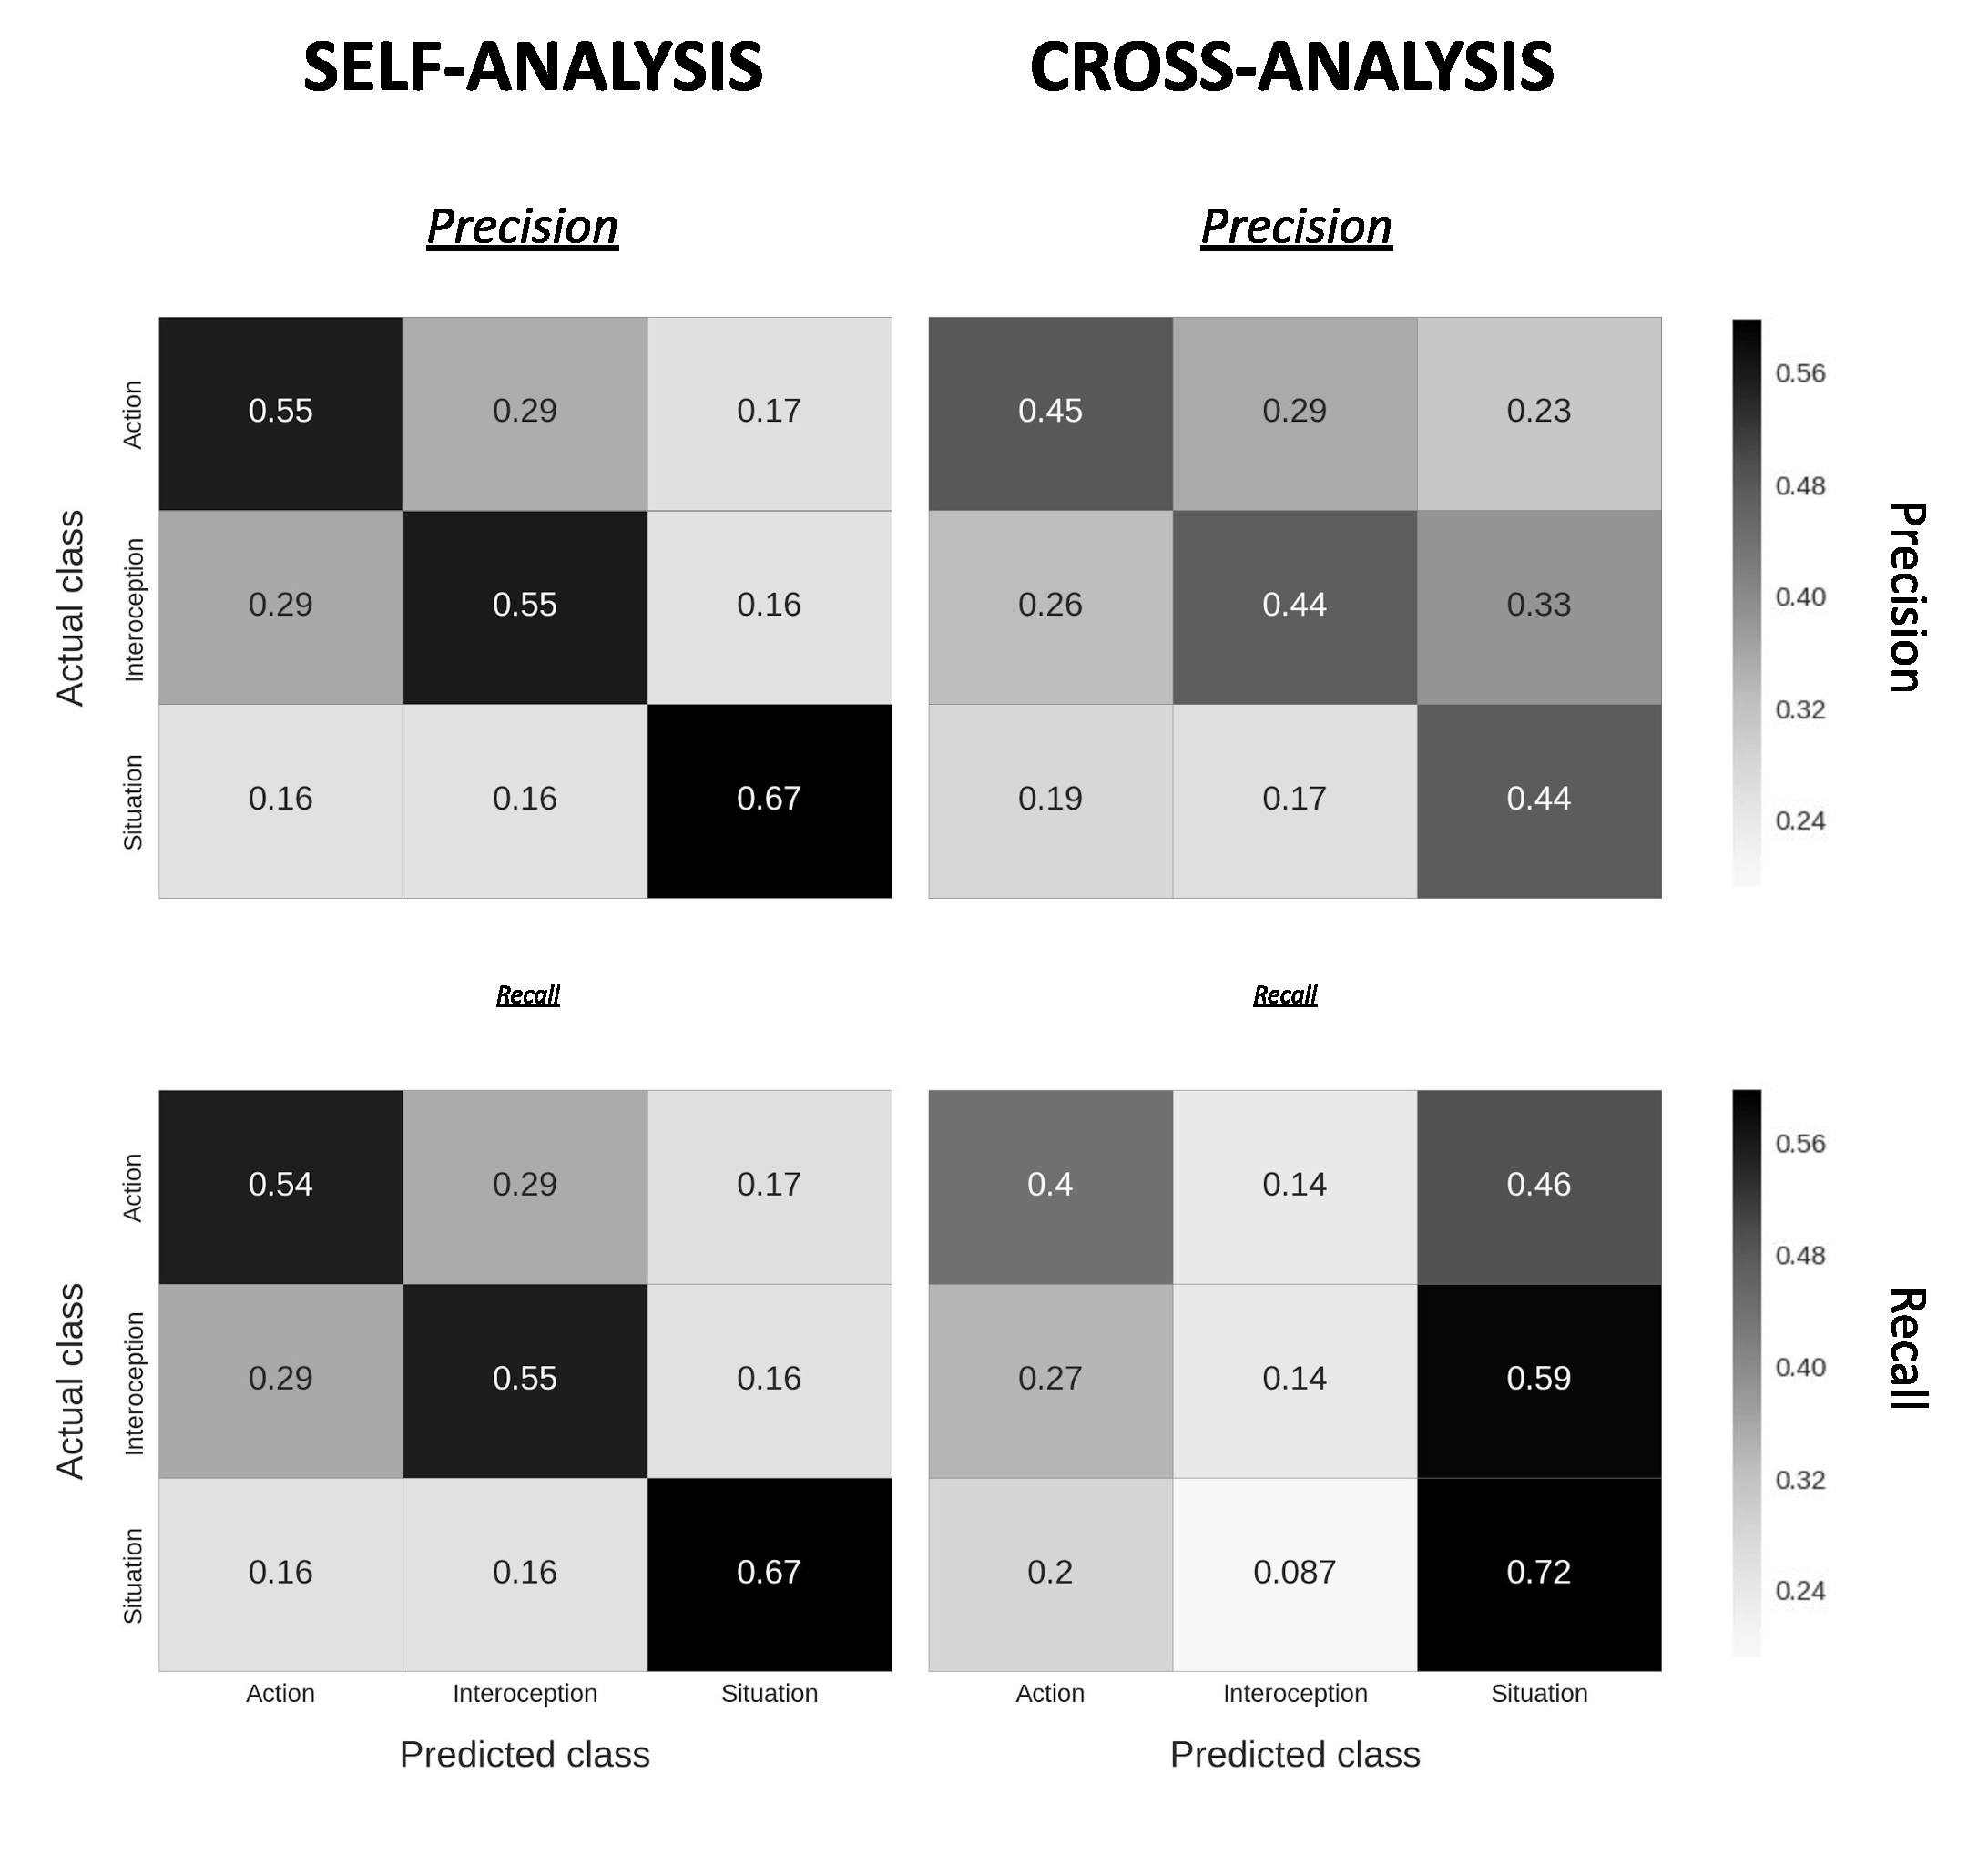
\includegraphics{_bookdown_files/shared-states-files/figures/figure_S5.pdf}
\caption{\label{fig:fig-shared-states-S5}A comparison between precision and recall confusion matrices of the self- and cross-analysis of the validation dataset. Precision refers to the amount of true positive predictions of a given class relative to all predictions for that class. Recall refers to the amount of true positive predictions of a given class relative to the total number of samples in that class. In the self-analysis, all classes were decoded significantly above chance for both precision and recall (all \emph{p} \textless{} 0.001). In the cross-analysis, all classes were decoded significantly above chance for precision (all \emph{p} \textless{} 0.001); for recall both action and situation were decoded significantly above chance (\emph{p} = 0.0013 and \emph{p} \textless{} 0.001, respectively), while interoception was decoded below chance. All \emph{p}-values were calculated using a permutation test with 1300 permutations (as described in the Methods section in the main text). When comparing precision and recall scores for both analyses, precision and recall showed very little differences in the self-analysis, while the cross-analysis shows a clear difference between metrics, especially for interoception and situation. For the interoception class, the relatively high precision score (44\%) compared to its recall score (14\%) suggests that trials are very infrequently classified as interoception, but when they are, it is (relatively) often correct. For the situation class, the relatively high recall score (72 \%) compared to its precision score (44\%) suggests that situation is strongly over-classified, which is especially clear in the lower-right confusion matrix, which indicates that 59\% of the interoception-trials are misclassified as situation-trials.}
\end{figure}



\newpage
\pagestyle{empty}

\hypertarget{self-vs.-other-classification}{%
\section{Self vs.~other classification}\label{self-vs.-other-classification}}

\begin{figure}
\centering
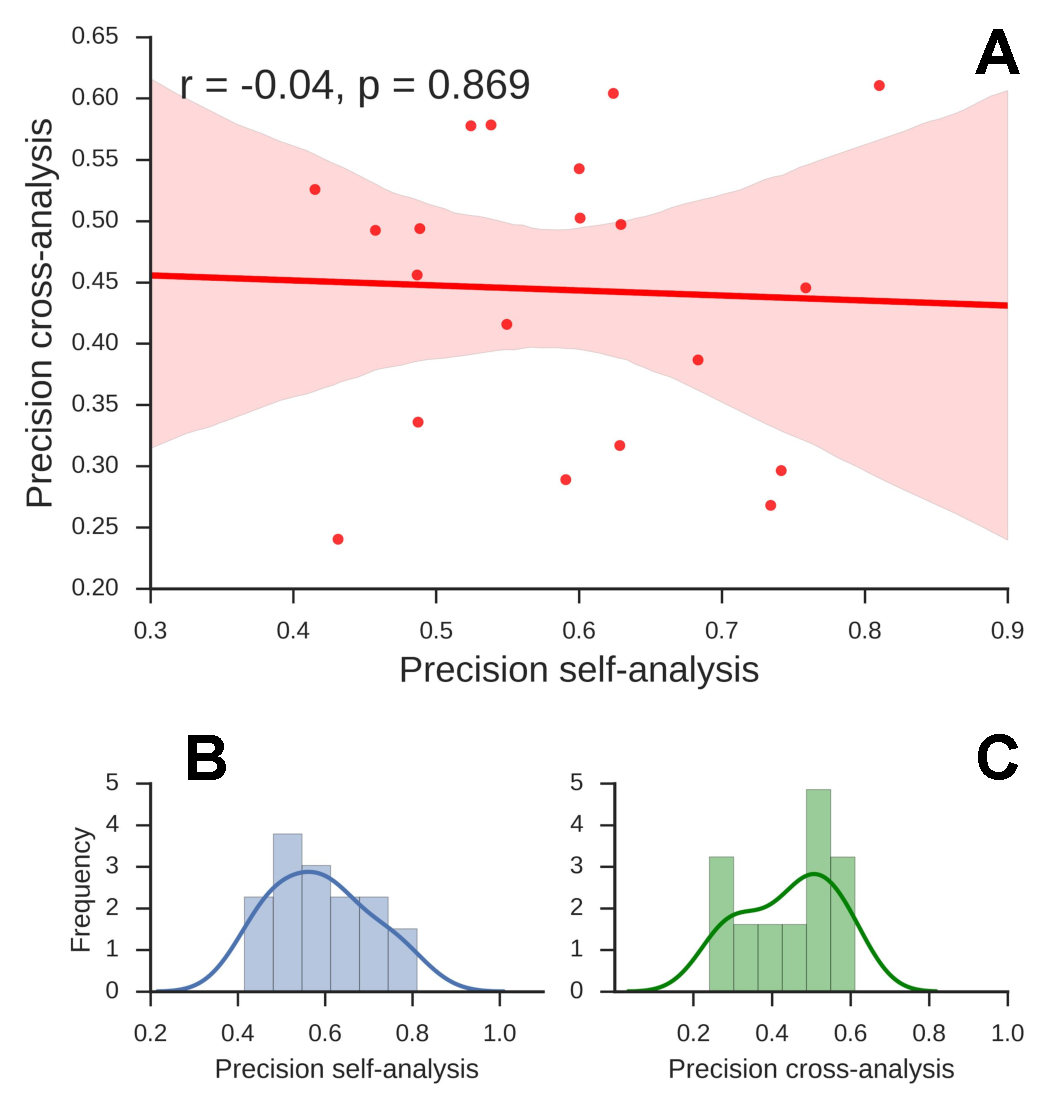
\includegraphics{_bookdown_files/shared-states-files/figures/figure_S6.pdf}
\caption{\label{fig:fig-shared-states-S6}Relation between self- and cross-analysis scores across subjects and their respective distributions. Note that the scores here represent the average of the class-specific precision scores. \textbf{A}) There is no significant correlation between precision-scores on the self-analysis and the corresponding scores on the cross-analysis, \emph{r} = -0.04, \emph{p} = .86, implying that classification scores in the self-analysis is not predictive of scores in the cross-analysis. \textbf{B}) The distribution of precision-scores in the self-analysis, appearing to be normally distributed. \textbf{C}) The distribution of precision-scores in the cross-analysis, on the other hand, appears to be bimodal, with one group of subjects having scores around chance level (0.333) while another group of subjects clearly scores above chance level (see individual scores and follow-up analyses in (ref:fig-shared-states-S4).}
\end{figure}



\newpage
\pagestyle{empty}

\hypertarget{self-to-other-cross-validation-results}{%
\section{Self-to-other cross-validation results}\label{self-to-other-cross-validation-results}}

\begin{figure}
\centering
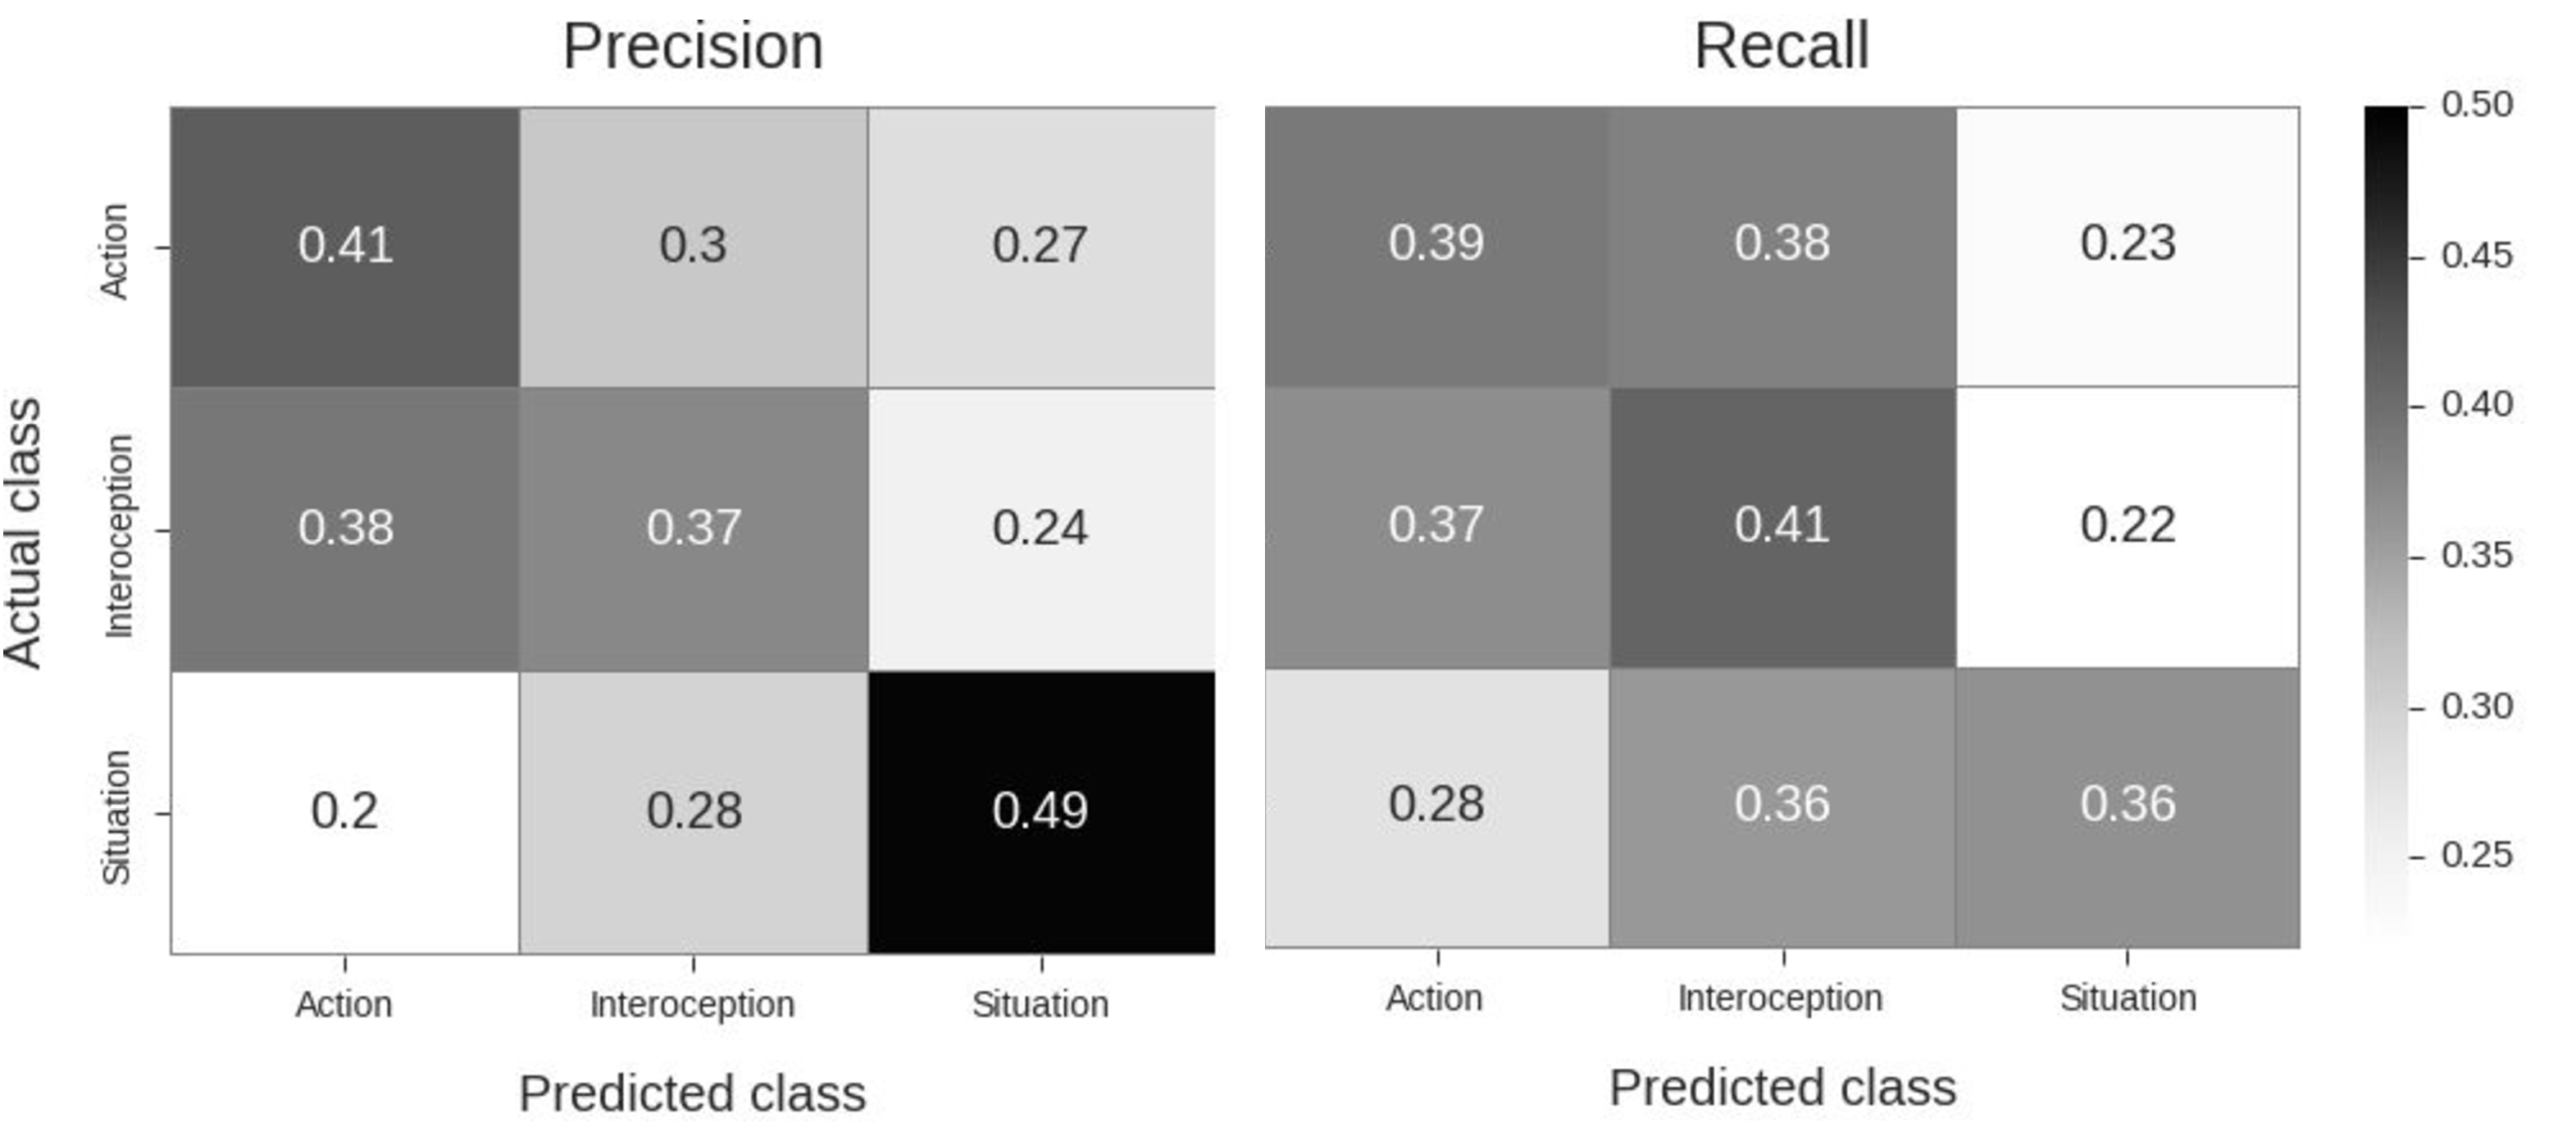
\includegraphics{_bookdown_files/shared-states-files/figures/figure_S7.pdf}
\caption{\label{fig:fig-shared-states-S7}Confusion matrices with precision (left matrix) and recall (right matrix) estimates of the other-to-self decoding analysis. The MVPA-pipeline used was exactly the same as for the (self-to-other) cross-analysis in the main text. \emph{P}-values corresponding to the classification scores were calculated using a permutation analysis with 1000 permutations of the other-to-self analysis with randomly shuffled class-labels. Similar to the self-to-other analysis, the precision-scores for all classes in the other-to-self analysis were significant, \emph{p}(action) \textless{} 0.001, \emph{p}(interoception) = 0.008, \emph{p}(situation) \textless{} 0.001. For recall, classification scores for action and interoception were significant (both \emph{p} \textless{} 0.001), but not significant for situation (\emph{p} = 0.062). The discrepancy between the self-to-other and other-to-self decoding analyses can be explained by two factors. First, the other-to-self classifier was trained on fewer samples (i.e.~90 trials) than the self-to-other classifier (which was trained on 120 trials), which may cause a substantial drop in power. Second, the preprocessing pipeline and MVPA hyperparameters were optimized based on the self-analysis and self-to-other cross-analysis. Given the vast differences between the nature of the self- and other-data, these optimal preprocessing and MVPA hyperparameters for the original analyses may not cross-validate well to the other-to-self decoding analysis.}
\end{figure}



\newpage
\pagestyle{empty}

\hypertarget{condition-average-results}{%
\section{Condition-average results}\label{condition-average-results}}

\begin{figure}
\centering
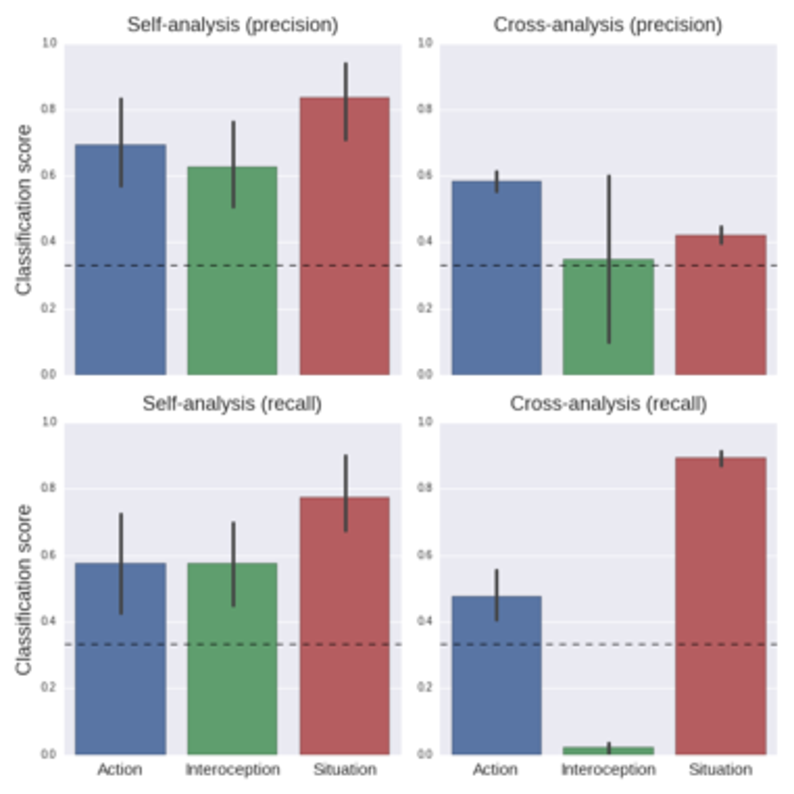
\includegraphics{_bookdown_files/shared-states-files/figures/figure_S8.pdf}
\caption{\label{fig:fig-shared-states-S8}Results of MVPA analyses using condition-average voxel patterns across subjects instead of single-trial patterns within subjects. Here, patterns are estimated in a GLM in which each condition, as opposed to each trial, is modeled with a single regressor, from which whole-brain t-value patterns were extracted. In this condition-average multi-voxel pattern analysis, condition-average patterns across subjects were used as samples. The condition-average patterns were extracted from the univariate first-level contrasts. In total, this yielded 120 samples for the self-data (3 conditions * 2 runs * 20 participants) and 60 samples for the other-data (3 conditions * 20 participants). For these analyses, the same hyperparameters were used as the original analyses reported in the main text, except with regard to the cross-validation and bagging procedure. Here, we used (stratified) 10-fold cross-validation without bagging. The upper panels show precision scores (per class) for the self- and (self-to-other) cross-analysis; the lower panels show results from the same analyses but expressed in recall-estimates (error bars indicate 95\% confidence intervals). Apart from interoception in the cross-analysis (both precision and recall), all scores were significant (p \textless{} 0.001) in a permutation test with 1000 permutations. These results largely replicate our findings as reported in the main text. This suggests that the neural patterns involved in self-focused emotional imagery and other-focused emotion understanding are relatively consistent in terms of spatial distribution across subjects. We explain this consistency by assuming that our tasks engage domain-general psychological processes that are present in all individuals.}
\end{figure}



\newpage
\pagestyle{empty}

\hypertarget{individual-subject-scores}{%
\section{Individual subject scores}\label{individual-subject-scores}}

\begin{table}

\caption{\label{tab:tab-shared-states-S3}Mean general classification scores (i.e., mean precision scores across action, interoception and situation) per subject for the self- and cross-analysis on the validation-set only.}
\centering
\resizebox{\linewidth}{!}{
\begin{tabular}[t]{rrrrl}
\toprule
Subject nr. & Self-analysis precision & Cross-analysis precision & Session & Part of optimization-set?\\
\midrule
1 & 0.758 & 0.445 & 2 & y\\
2 & 0.487 & 0.336 & 2 & y\\
3 & 0.629 & 0.316 & 1 & y\\
4 & 0.524 & 0.577 & 2 & y\\
5 & 0.457 & 0.492 & 1 & y\\
\addlinespace
6 & 0.741 & 0.296 & 2 & y\\
7 & 0.600 & 0.542 & 1 & y\\
8 & 0.431 & 0.240 & 2 & y\\
9 & 0.629 & 0.497 & 1 & y\\
10 & 0.734 & 0.268 & 2 & y\\
\addlinespace
11 & 0.683 & 0.386 & 1 & y\\
12 & 0.415 & 0.525 & 2 & y\\
13 & 0.623 & 0.604 & 1 & y\\
14 & 0.810 & 0.610 & 1 & n\\
15 & 0.538 & 0.578 & 1 & n\\
\addlinespace
16 & 0.486 & 0.455 & 1 & n\\
17 & 0.549 & 0.415 & 1 & n\\
18 & 0.488 & 0.494 & 1 & n\\
19 & 0.590 & 0.289 & 1 & n\\
20 & 0.600 & 0.502 & 1 & n\\
\bottomrule
\multicolumn{5}{l}{\rule{0pt}{1em}\textit{Note: } Supplementary Table 3 suggests individual variability in the extent to which neural resources are shared between self- and other-focused processes. In the SF-task all subjects demonstrated a mean classification score well above .33 (i.e., score associated with chance). When generalizing the SF-classifier to the OF-task, however, the classification scores appear to be bimodally distributed (see Supplementary Figure 5C). As can be seen in Table 3, some subjects demonstrated a relatively high mean classification score (i.e., > .45), whereas other subjects demonstrated a classification score at chance level or lower. Note that there is no significant difference between the OF classification scores for subjects who participated in the experiment for the first or second time (“Session” column in table; *t*(18) = 1.73, p = 0.10), nor for subjects who were or were not part of the optimization-set (“Part of optimization-set?” column in table; *t*(18) = -.95, p = 0.35), suggesting that inclusion in the optimization-set or session ordering is not a confound in the analyses. Regarding individual variability in self-other neural overlap, it is important to note that in the field of embodied cognition, there is increasing attention for the idea that simulation is both individually and contextually dynamic (Oosterwijk \& Barrett, 2014; Winkielman, Niedenthal, Wielgosz \& Kavanagh, 2015; see also Barrett, 2009). To better distinguish between meaningful individual variation and variation due to other factors (e.g., random noise), future research should test a priori formulated hypotheses about how and when individual variation is expected to occur. }\\
\end{tabular}}
\end{table}

\newpage
\pagestyle{empty}

\hypertarget{brain-region-importance}{%
\section{Brain region importance}\label{brain-region-importance}}

\begin{table}

\caption{\label{tab:tab-shared-states-S4}Most important voxels in terms of their average weight across iterations and subjects.}
\centering
\resizebox{\linewidth}{!}{
\begin{tabular}[t]{lrrrr}
\toprule
Brain region & k & Max & Mean & Std\\
\midrule
Frontal pole & 1827 & 5.05 & 2.35 & 0.52\\
Occipital pole & 1714 & 5.15 & 2.45 & 0.56\\
Supramarginal gyrus anterior & 1573 & 7.48 & 2.84 & 0.91\\
Lateral occipital cortex superior & 1060 & 4.52 & 2.18 & 0.39\\
Lateral occipital cortex inferior & 923 & 4.73 & 2.36 & 0.49\\
\addlinespace
Angular gyrus & 856 & 4.52 & 2.24 & 0.40\\
Supramarginal gyrus posterior & 806 & 4.49 & 2.29 & 0.45\\
Middle temporal gyrus temporo-occipital & 798 & 4.00 & 2.33 & 0.48\\
Temporal pole & 711 & 4.38 & 2.37 & 0.54\\
Precentral gyrus & 568 & 3.54 & 2.14 & 0.31\\
\addlinespace
Superior temporal gyrus posterior & 549 & 3.64 & 2.27 & 0.41\\
Superior frontal gyrus & 510 & 3.83 & 2.18 & 0.38\\
Postcentral gyrus & 489 & 4.61 & 2.43 & 0.60\\
Inferior frontal gyrus parstriangularis & 488 & 4.22 & 2.35 & 0.50\\
Inferior frontal gyrus parsopercularis & 441 & 3.54 & 2.14 & 0.31\\
\addlinespace
Middle temporal gyrus posterior & 417 & 5.68 & 2.34 & 0.52\\
Occipital fusiform & 400 & 4.28 & 2.14 & 0.37\\
Middle temporal gyrus anterior & 398 & 5.68 & 2.58 & 0.76\\
Middle frontal gyrus & 300 & 3.01 & 2.06 & 0.25\\
Precuneus & 282 & 3.34 & 2.14 & 0.31\\
\bottomrule
\multicolumn{5}{l}{\rule{0pt}{1em}\textit{Note: } Brain regions were extracted from the Harvard-Oxford (bilateral) Cortical atlas. A minimum threshold for the probabilistic masks of 20 was chosen to minimize overlap between adjacent masks while maximizing coverage of the entire brain. The column *k* represents the absolute number of above-threshold voxels in the masks. The columns *Max*, *Mean*, and *Std* represent the maximum, mean, and standard deviation from the *t*-values included in the masks. Note that the *t*-values, corresponding to the mean weight across subjects normalized by the standard error of the weights across subjects (after correcting for a positive bias when taking the absolute of the weights), were thresholded at a minimum of 1.75, referring to a *p*-value of 0.05 of a one-sided *t*-test against zero with 19 degrees of freedom (i.e. *n* – 1). Note that this *t*-value map was not corrected for multiple comparisons, and is intended to visualize which regions in the brain were generally involved in our sample of subjects. The *X*, *Y*, and *Z* columns represent the MNI152 (2mm) coordinates of the peak (i.e. max) *t*-value for each listed brain region.}\\
\end{tabular}}
\end{table}

\hypertarget{general-note-about-tables-with-voxel-coordinates}{%
\section{General note about tables with voxel-coordinates}\label{general-note-about-tables-with-voxel-coordinates}}

In order to keep the Supplementary materials concise and orderly, we chose not to include the actual tables with the peak coordinates of all significant clusters of the univariate analyses of the self- and other-task data (as these would amount to 25 pages). These tables, however, can be downloaded (as simple tab-separated-value files) from the study's \href{https://github.com/lukassnoek/SharedStates}{Github respository}. The voxel tables are listed under: \texttt{SharedStates/RESULTS/Voxel\_tables/*.tsv} (see green box in image below), and can be downloaded by cloning the remote Github repository locally or downloading the ZIP-file from the website (see red box in image below).

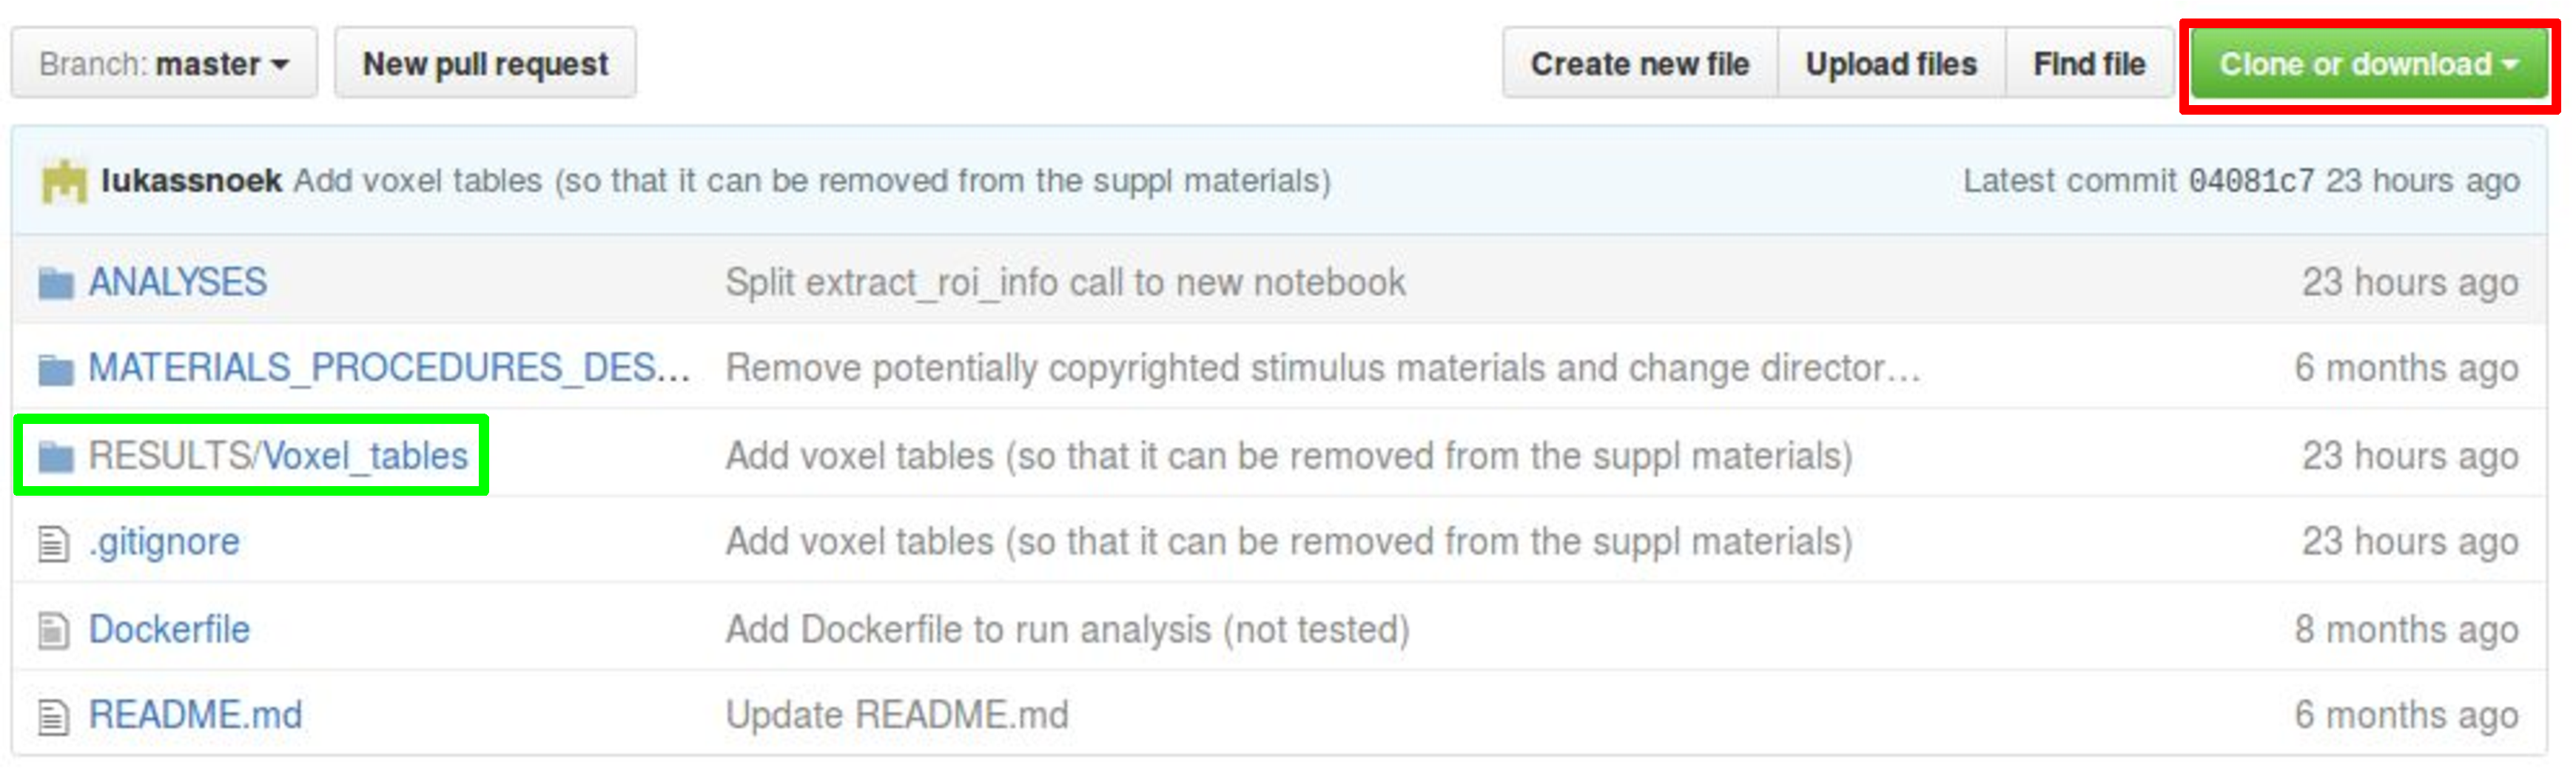
\includegraphics{_bookdown_files/shared-states-files/figures/github.pdf}

\hypertarget{confounds-decoding-supplement}{%
\chapter{Supplement to Chapter \ref{confounds-decoding}}\label{confounds-decoding-supplement}}

\hypertarget{morbid-curiosity-supplement}{%
\chapter{Supplement to Chapter \ref{morbid-curiosity}}\label{morbid-curiosity-supplement}}

\hypertarget{au-limitations-supplement}{%
\chapter{Supplement to Chapter \ref{au-limitations}}\label{au-limitations-supplement}}

\hypertarget{facial-expression-models-supplement}{%
\chapter{Supplement to Chapter \ref{facial-expression-models}}\label{facial-expression-models-supplement}}

\hypertarget{resources-supplement}{%
\chapter{Data, code and materials}\label{resources-supplement}}

\backmatter

\hypertarget{bibliography}{%
\chapter*{Bibliography}\label{bibliography}}
\addcontentsline{toc}{chapter}{Bibliography}

\markboth{\MakeUppercase{Bibliography}}{} % have to explicitly state what to put in the heading (bug in bookdown?)
%format the references so they have a hanging indent. Remove these (and the \endgroup command) if you want regular indentation.
\begingroup
\hspace{\parindent}
\setlength{\parindent}{-0.25in}
\setlength{\leftskip}{0.25in}
\setlength{\parskip}{0pt}

\hypertarget{refs}{}

\endgroup

\hypertarget{contributions-to-the-chapters}{%
\chapter*{Contributions to the chapters}\label{contributions-to-the-chapters}}
\addcontentsline{toc}{chapter}{Contributions to the chapters}

\chaptermark{Contributions to chapters}
\setlength{\parindent}{0pt}
\small

\hypertarget{list-of-other-publications}{%
\chapter*{List of other publications}\label{list-of-other-publications}}
\addcontentsline{toc}{chapter}{List of other publications}

\chaptermark{List of other publications}

Alilović, J., Timmermans, B., \textbf{Reteig, L. C.}, van Gaal, S., \& Slagter, H. A. (2019). No evidence that predictions and attention modulate the first feedforward sweep of cortical information processing. \emph{Cerebral Cortex, 29} 2261--2278. \url{https://doi.org/10.1093/cercor/bhz038}\newline

van Schouwenburg, M. R., Sörensen, L. K. A., de Klerk, R., \textbf{Reteig, L. C.}, \& Slagter, H. A. (2018). No differential effects of two different alpha-band electrical stimulation protocols over fronto-parietal regions on spatial attention. \emph{Frontiers in Neuroscience} 12:433. \url{https://doi.org/10.3389/fnins.2018.00433}\newline

Slagter, H. A., Mazaheri, A., \textbf{Reteig, L. C.}, Smolders, R., Figee, M., Mantione, M., \ldots{} Denys, D. (2017). Contributions of the Ventral Striatum to Conscious Perception: An Intracranial EEG Study of the Attentional Blink. \emph{Journal of Neuroscience, 37}, 1081--1089. \url{https://doi.org/10.1523/jneurosci.2282-16.2016}\newline

Slagter, H. A., Prinssen, S., \textbf{Reteig, L. C.}, \& Mazaheri, A. (2016). Facilitation and inhibition in attention: Functional dissociation of pre-stimulus alpha activity, P1, and N1 components. \emph{NeuroImage, 125}, 25--35. \url{https://doi.org/10.1016/j.neuroimage.2015.09.058}

\normalsize
\setlength{\parindent}{1.5em}

\hypertarget{nederlandse-samenvatting-summary-in-dutch}{%
\chapter*{Nederlandse samenvatting (Summary in Dutch)}\label{nederlandse-samenvatting-summary-in-dutch}}
\addcontentsline{toc}{chapter}{Nederlandse samenvatting (Summary in Dutch)}

\chaptermark{Summary in Dutch}

\begin{dutch}

\emph{Replace this with the Dutch title of your thesis}

\bigskip

The summary goes here.

\end{dutch}

\hypertarget{acknowledgments}{%
\chapter*{Acknowledgments}\label{acknowledgments}}
\addcontentsline{toc}{chapter}{Acknowledgments}

\chaptermark{Acknowledgments}

This section is optional, but theses typically include acknowledgments (\textdutch{\emph{dankwoord}} in Dutch) at the end. You may want to mix languages to thank people in their native tongue (though most Dutch speakers write it entirely in Dutch). But the standard language of the thesis template is English. You can switch temporarily by wrapping the text in language tags like so: \texttt{{[}Your\ Dutch\ text\ here{]}\{lang=nl\}}. This is important for things like hyphenation to work properly.

\backmatter
\printbibliography


\end{document}
